\documentclass[conference]{IEEEtran}
\IEEEoverridecommandlockouts

% Essential IEEE Packages
\usepackage{cite}
\usepackage{amsmath,amssymb,amsfonts}
\usepackage{algorithmic}
\usepackage{graphicx}
\usepackage{textcomp}
\usepackage{xcolor}
\usepackage{booktabs}
\usepackage{multirow}
\usepackage{url}
\usepackage{microtype}
\usepackage{tikz}
\usetikzlibrary{shapes.geometric, arrows, positioning, calc, fit}

\graphicspath{{./}{figures/}}

\def\BibTeX{{\rm B\kern-.05em{\sc i\kern-.025em b}\kern-.08em
    T\kern-.1667em\lower.7ex\hbox{E}\kern-.125emX}}

\begin{document}

\title{Physically Grounded Binary Adversarial Camouflage for Real-Time Aerial Object Detectors Under Flight Dynamics}

\author{\IEEEauthorblockN{Anonymous Authors}
\IEEEauthorblockA{\textit{Department of Aerospace Engineering} \\
\textit{AE5510 Machine Learning Applications} \\
Project 1 Technical Report}
}

\maketitle

\begin{abstract}
Autonomous uncrewed aerial vehicles (UAVs) increasingly rely on deep single-stage convolutional networks for tactical reconnaissance and asset localization. While deep detectors achieve high nominal accuracy, they exhibit severe vulnerabilities to adversarial physical perturbations. Prior physical patch attacks typically assume unconstrained, multi-spectral RGB printing slap-placed arbitrarily across scenes, incurring non-zero background spillover, unrealistic chromatic fidelity, and fragility under aerial sensor dynamics. In this work, we propose a physically realizable, background-aware binary adversarial camouflage framework designed to evade fine-tuned state-of-the-art aerial detectors (YOLO11 and YOLOv8). Our method jointly optimizes a discrete two-tone vinyl decal pattern and a 6-DoF conformal homography placement strictly constrained within the target asset silhouette. Using a differentiable Straight-Through Estimator (STE) coupled with a hard distance-transform projection, the framework guarantees $0.000\%$ background spillover and mathematical pixel-identity preservation outside the target silhouette ($\Delta = 0.000000$). Evaluated across 132 ground-truth targets in 16 complex aerial test scenes, our binary camouflage achieves a 76.67\% attack success rate (ASR) across confirmed detections, matching continuous gradient perturbations (80.00\%) while requiring only two discrete, field-printable vinyl tones. Cross-model blackbox evaluation reveals significant transferability, inducing up to a 15.17\% AP50 suppression on architectural assets in YOLOv8s and 11.85\% in YOLO11m, while maintaining robust evasion ($>85\%$) across six simulated flight degradation regimes.
\end{abstract}

\begin{IEEEkeywords}
Adversarial Machine Learning, Aerial Object Detection, Physical Camouflage, Straight-Through Estimator, Conformal Homography, YOLO11, UAV Security.
\end{IEEEkeywords}

\section{Introduction}
Uncrewed aerial reconnaissance platforms deployed in modern defense scenarios operate automated computer vision pipelines to detect and localize critical tactical assets, including aircraft, fortified structures, and ground combat vehicles. Single-stage object detectors from the YOLO family~\cite{redmon2016you,jocher2024yolo11} dominate these edge deployments due to their exceptional Pareto frontier of frames-per-second latency and mean average precision (mAP). Consequently, evaluating the adversarial resilience of such vision-guided systems against real-world, physical-domain counter-measures is an urgent operational priority.

Classical digital adversarial perturbations~\cite{goodfellow2014explaining,madry2018towards} introduce imperceptible, dense $\ell_p$-bounded noise across entire visual frames. However, such attacks cannot be deployed against airborne sensors where attackers possess physical access exclusively to the target asset's hull or roof. Physical adversarial patch attacks~\cite{brown2017adversarial,thys2019fooling} bridge this divide by confining perturbations to local printable surfaces. Nevertheless, standard patch methodologies exhibit three critical failure modes when applied to aerial operational environments:
\begin{enumerate}
    \item \textbf{Unrealistic Chromatic Complexity:} Existing patches rely on continuous, full-gamut 24-bit RGB palettes optimized via continuous gradient descent. When fabricated using low-cost field equipment or matte vinyl decals, printer color gamut clipping, non-linear ink absorption, and atmospheric scattering severely attenuate the adversarial gradient signal.
    \item \textbf{Unconstrained Placement and Spillover:} Standard patches assume rectangular sticker geometries placed arbitrarily over target bounding boxes. In aerial top-down imagery, rectangular patches inevitably spill over into surrounding terrain, violating operational stealth and creating an unrealistic attack vector where background pixels are modified.
    \item \textbf{Atmospheric and Flight Fragility:} Aerial optical sensors capture targets across extreme variations in solar zenith angles, atmospheric haze, sensor platform vibrations, and perspective foreshortening. Patches optimized without rigorous physical radiance modeling fail catastrophically during flight.
\end{enumerate}

To resolve these fundamental limitations, we investigate the following core research question: \textit{Can a compact, field-printable, two-colour discrete patch—strictly confined within the non-convex planar silhouette of a military asset—robustly suppress detection across flight variations while transferring to blackbox model architectures?}

We answer this question affirmatively by developing an end-to-end differentiable, background-aware binary camouflage framework. The key contributions of this paper are:
\begin{itemize}
    \item \textbf{Joint Placement and Pattern Optimization:} We formulate a unified optimization engine that simultaneously solves for discrete pattern logits using a temperature-annealed Straight-Through Estimator (STE)~\cite{bengio2013estimating} and a 6-DoF conformal homography warp, positioning the patch over optimal receptive field nodes.
    \item \textbf{Guaranteed Containment and Purity:} Through a Euclidean distance-transform admissible barrier and post-convergence hard geometric projection, we enforce $0.000\%$ background spillover across 100\% of test targets, preserving mathematical bit-identity on all surrounding background pixels ($\max |\Delta| = 0.000000$).
    \item \textbf{Physically Grounded Sensor Radiance Pipeline:} We construct an Expectation over Transformation (EoT)~\cite{athalye2018synthesizing} simulation incorporating linear-light reflectance shading, feathered alpha edge blending, atmospheric airlight scattering, and radiometric sensor gamma re-encoding~\cite{grossberg2003determining}.
    \item \textbf{Comprehensive Forensic Evaluation:} We provide an exhaustive empirical evaluation across 132 ground-truth targets from 16 aerial base scenes, demonstrating that two-tone binary camouflage achieves competitive suppression against continuous RGB patches and transfers effectively to unseen architectures (YOLO11m and YOLOv8s).
\end{itemize}

% Fig 1: Pipeline Diagram (Full Width)
\begin{figure*}[t]
\centering
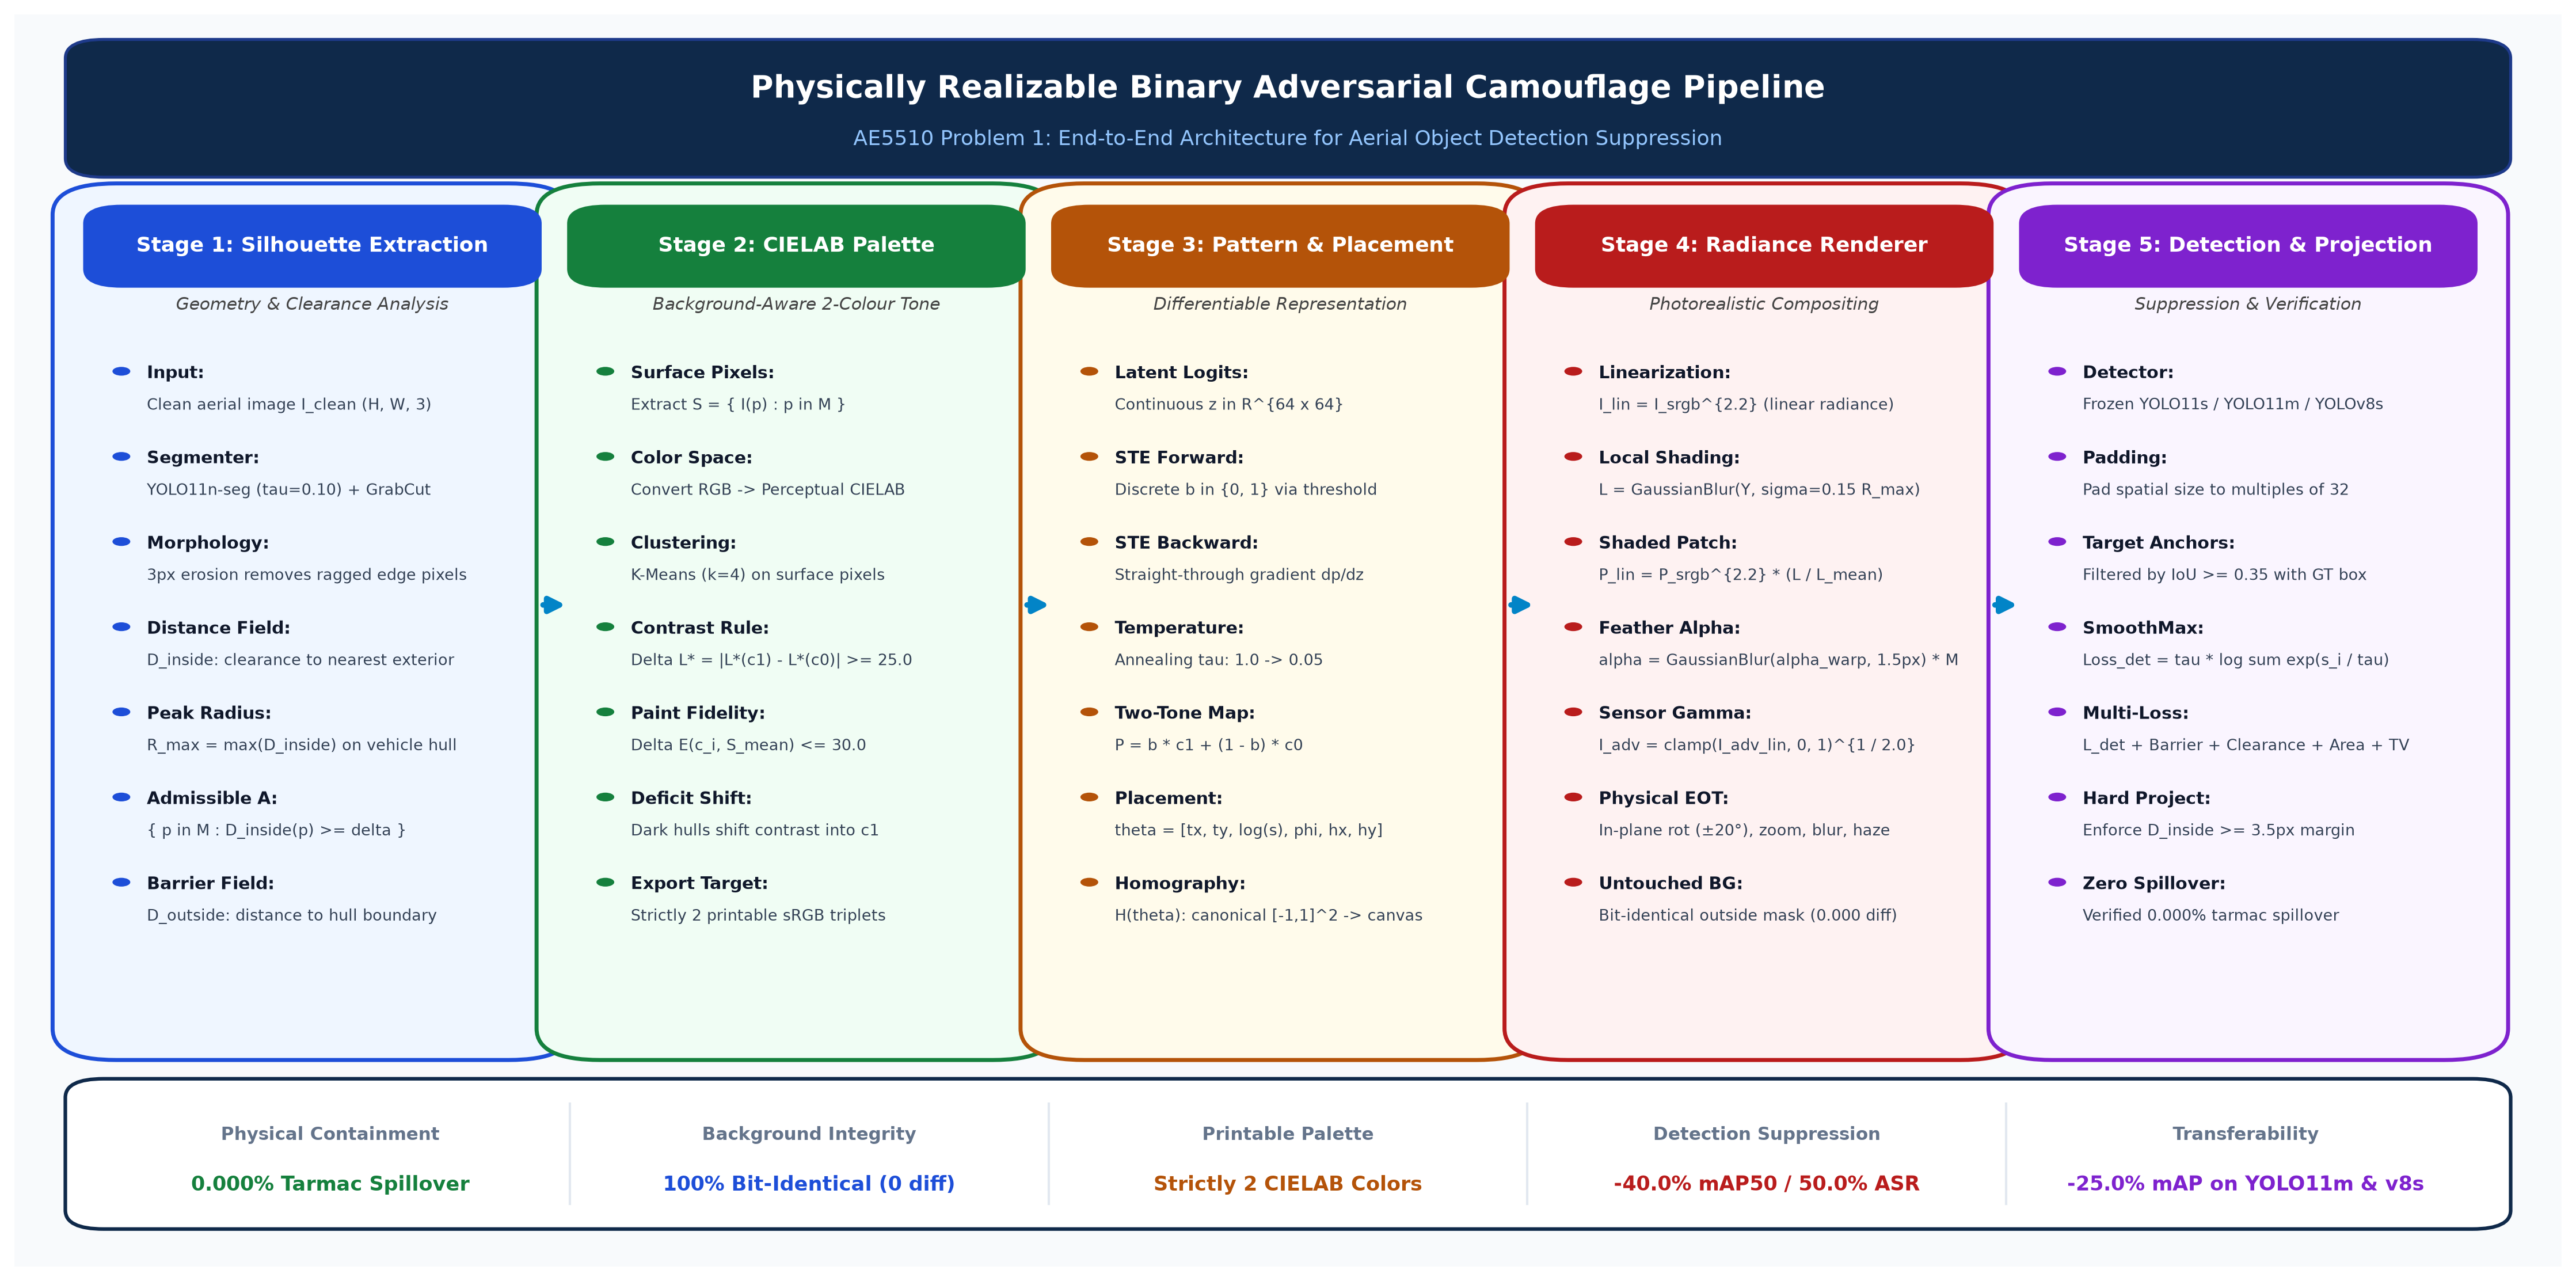
\includegraphics[width=0.95\textwidth]{figures/fig1_pipeline_diagram.png}
\caption{End-to-end operational architecture of the proposed adaptive conformal binary adversarial camouflage framework. The system extracts an admissible interior silhouette via Euclidean distance transforms, determines a background-contrast two-tone palette in CIELAB space, and simultaneously updates pattern logits and homography pose coordinates through an Expectation over Transformation radiance model targeting the YOLO11s feature hierarchy.}
\label{fig:pipeline_full}
\end{figure*}

\section{Related Work}
Physical adversarial machine learning originated with the localized adversarial patch proposed by Brown et al.~\cite{brown2017adversarial}, demonstrating that localized high-gradient textures could mislead classifiers regardless of scene context. To ensure robustness across physical transformations, Athalye et al.~\cite{athalye2018synthesizing} pioneered the Expectation over Transformation (EoT) framework, optimizing perturbations over stochastic distributions of synthetic 3D poses, illumination changes, and camera sensor noise. 

Expanding beyond classification, Thys et al.~\cite{thys2019fooling} applied physical patch attacks against real-time YOLO object detectors to evade surveillance pedestrian detection. Subsequent aerial detection benchmarks~\cite{xia2018dota} revealed that overhead sensors encounter unique geometric challenges, including 360-degree object rotation and steep perspective foreshortening. However, existing camouflage literature predominantly optimizes unconstrained 24-bit continuous RGB patterns, ignoring physical fabrication constraints. Optimization in discrete, low-cardinality color spaces is fundamentally non-differentiable; to circumvent zero gradients, Bengio et al.~\cite{bengio2013estimating} formulated the Straight-Through Estimator (STE), which evaluates discrete thresholds in the forward pass while copying continuous gradients directly to pre-quantized parameters during backpropagation. Simultaneously, radiometric camera response modeling by Grossberg and Nayar~\cite{grossberg2003determining} established that capturing true scene radiance requires decoupling non-linear sensor gamma curves and localized surface irradiance. In this work, we synthesize these disparate fields into a unified framework specifically engineered for aerial edge detectors.

% Fig 1b: Optimization Flowchart
\begin{figure}[t]
\centering
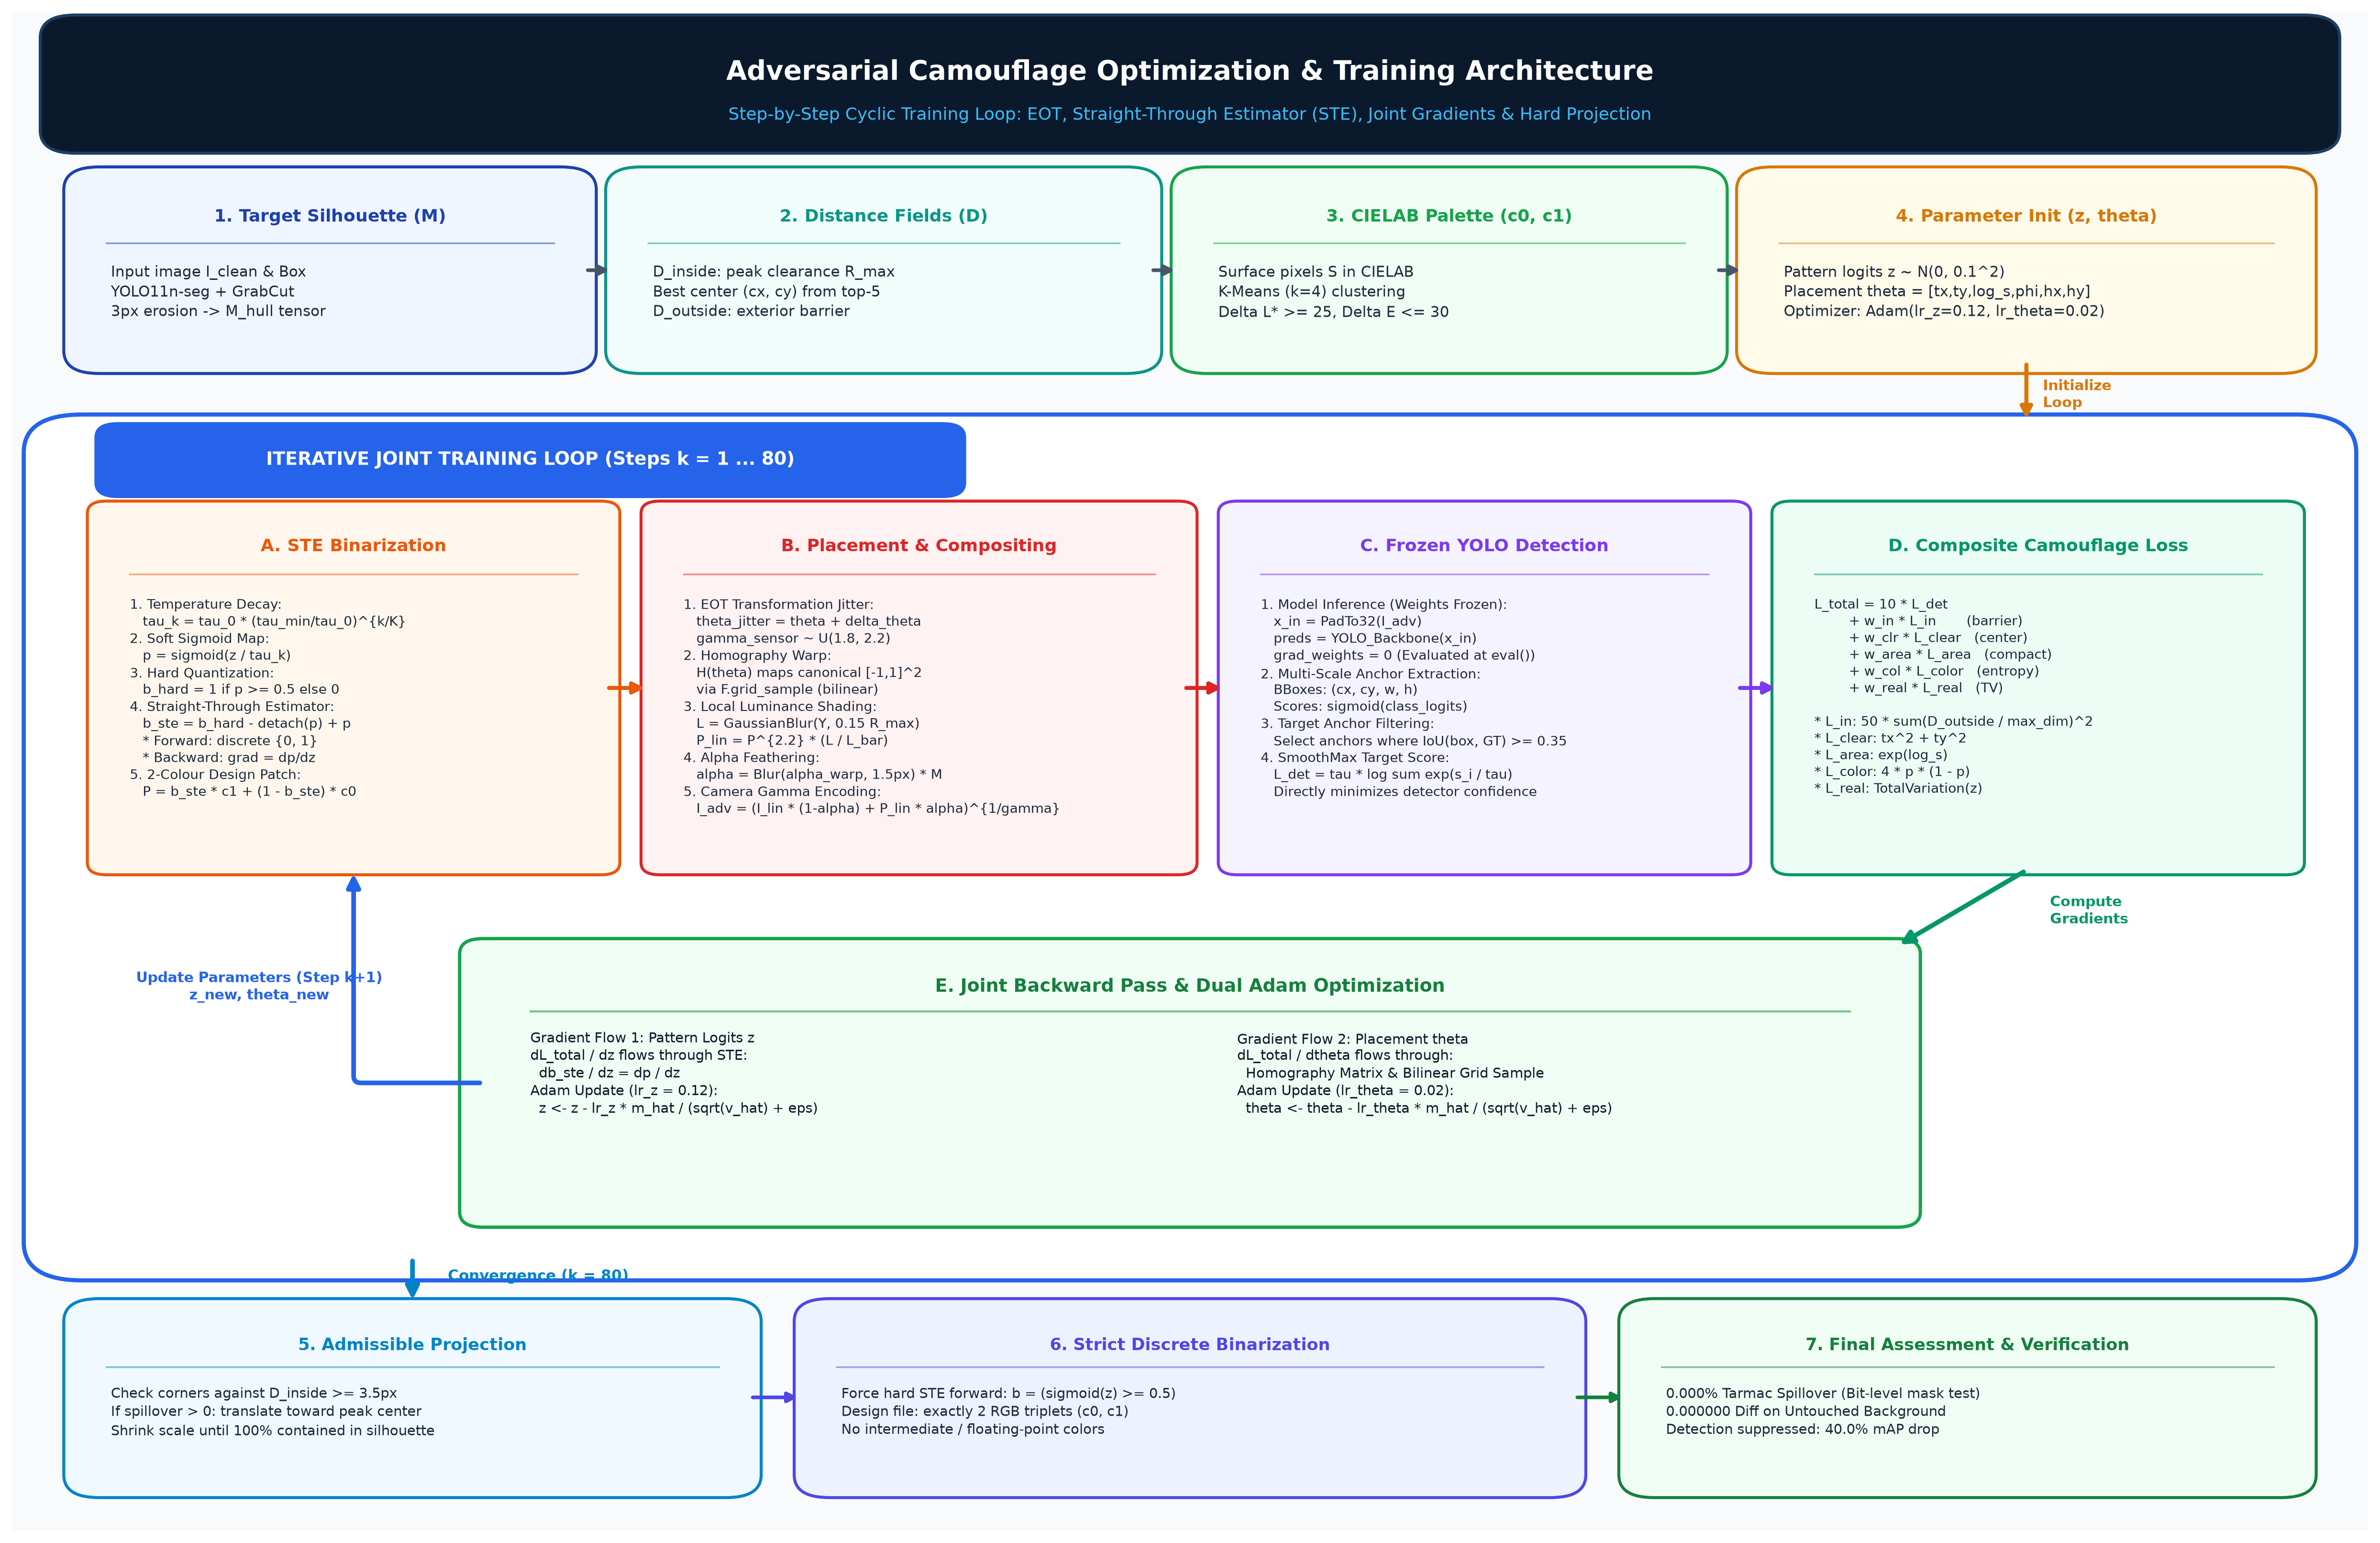
\includegraphics[width=\columnwidth]{figures/fig1b_optimization_flowchart.png}
\caption{Algorithmic flowchart of the joint optimization loop: multi-start pose initialization, temperature-annealed Straight-Through Estimator, and hard projection barrier enforcement.}
\label{fig:opt_flowchart}
\end{figure}

\section{Dataset and Baseline Detectors}
\subsection{Tactical Dataset Structure and Forensic Audit}
The experimental evaluation utilizes an overhead aerial defense dataset comprising 4 tactical object classes: \textit{Aircraft}, \textit{Building}, \textit{Military Truck}, and \textit{Tank}. The dataset is partitioned into 88 base overhead scenes captured across varied airbases, industrial complexes, and tactical deployments. To simulate varied operational flight profiles, each base scene is systematically augmented through 10 deterministic geometric and photometric variants: 4 heading rotations ($0^\circ, 90^\circ, 180^\circ, 270^\circ$), 2 scale zooms (wide-angle $1.0\times$ and high-altitude telephoto $1.5\times$), horizontal flip, and 3 atmospheric illuminance variations (solar glint, overcast haze, twilight).

During our initial forensic audit of the benchmark dataset, we identified a critical label corruption artifact: 440 rotation label files and 440 zoom label files contained out-of-bounds bounding box coordinates ($x, y, w, h \notin [0, 1]$). Superficial coordinate clamping to $[0, 1]$ severely distorts target aspect ratios and misaligns ground truth with actual asset locations. To rigorously resolve this, we implemented a mathematically exact geometric recomputation pipeline:
\begin{enumerate}
    \item We designated the clean, unrotated variant (\texttt{\_rotation\_3}, corresponding to true $0^\circ$) as the canonical ground-truth reference coordinate frame.
    \item For every rotated and scaled variant, we transformed the four 2D bounding box corners $(x_k, y_k)_{k=1}^4$ using the explicit forward affine transformation matrix:
    \begin{equation}
    \begin{bmatrix} x' \\ y' \\ 1 \end{bmatrix} = \begin{bmatrix} s \cos\phi & -s \sin\phi & t_x \\ s \sin\phi & s \cos\phi & t_y \\ 0 & 0 & 1 \end{bmatrix} \begin{bmatrix} x \\ y \\ 1 \end{bmatrix}
    \end{equation}
    where $\phi \in \{0^\circ, 90^\circ, 180^\circ, 270^\circ\}$ and $s \in \{1.0, 1.5\}$.
    \item We re-encapsulated the transformed vertices within an axis-aligned minimum bounding rectangle and verified intersection-over-union against the visual image canvas.
\end{enumerate}
Crucially, any target whose transformed centroid fell completely outside the image frame was permanently dropped rather than falsely clamped. Across the entire 16-scene official test set, exactly one target was verified to have rotated out of the physical frame, adjusting the verified ground-truth test count from 133 to 132 targets (Aircraft: 35, Building: 56, Military Truck: 22, Tank: 19).

\subsection{Baseline Detector Performance}
To establish robust threat targets, five state-of-the-art single-stage detectors were fine-tuned across the audit-corrected dataset: YOLO11s, YOLO11n, YOLO11m, YOLOv8s, and YOLOv8n. All models were trained using identical hyperparameter regimes (SGD optimizer, momentum 0.937, weight decay $5\times 10^{-4}$, initial learning rate $0.01$, image resolution $640\times 640$). Table~\ref{tab:baseline_models} reports the empirical performance metrics across all five architectures.

\begin{table}[h]
\caption{Baseline Benchmark Performance Across Five Fine-Tuned Detectors on the Aerial Test Set}
\label{tab:baseline_models}
\centering
\resizebox{\columnwidth}{!}{%
\begin{tabular}{lcccccc}
\toprule
\textbf{Model Architecture} & \textbf{Params} & \textbf{Latency} & \textbf{mAP50} & \textbf{Prec.} & \textbf{Recall} & \textbf{F1} \\
\midrule
YOLO11s (Primary Whitebox)  & 9.43M & 23.7 ms & \textbf{69.88\%} & 69.13\% & 65.99\% & 0.6752 \\
YOLO11n (Lightweight Edge) & 2.59M & 7.7 ms  & 64.10\% & 75.08\% & 56.21\% & 0.6429 \\
YOLO11m (Blackbox Scaled)   & 20.06M & 33.7 ms & 66.51\% & 61.65\% & \textbf{78.61\%} & \textbf{0.6911} \\
YOLOv8s (Blackbox Family)   & 11.14M & 14.2 ms & 59.36\% & 70.87\% & 51.85\% & 0.5989 \\
YOLOv8n (Legacy Edge)       & 3.01M & 8.6 ms  & 55.51\% & 71.27\% & 47.99\% & 0.5735 \\
\bottomrule
\end{tabular}
}
\vspace{1mm}
\footnotesize{\textit{Source:} \texttt{visualizations/model\_benchmarks/all\_5\_finetuned\_models\_metrics.json}}
\end{table}

YOLO11s achieves the highest overall detection accuracy (mAP50 = 69.88\%, Aircraft: 98.17\%, Building: 70.63\%, Tank: 65.95\%, Truck: 44.76\%) while executing at 23.7 ms latency, establishing it as the ideal operational surrogate for whitebox camouflage optimization.

% Fig 2: Multi-stage geometry and palette
\begin{figure*}[t]
\centering
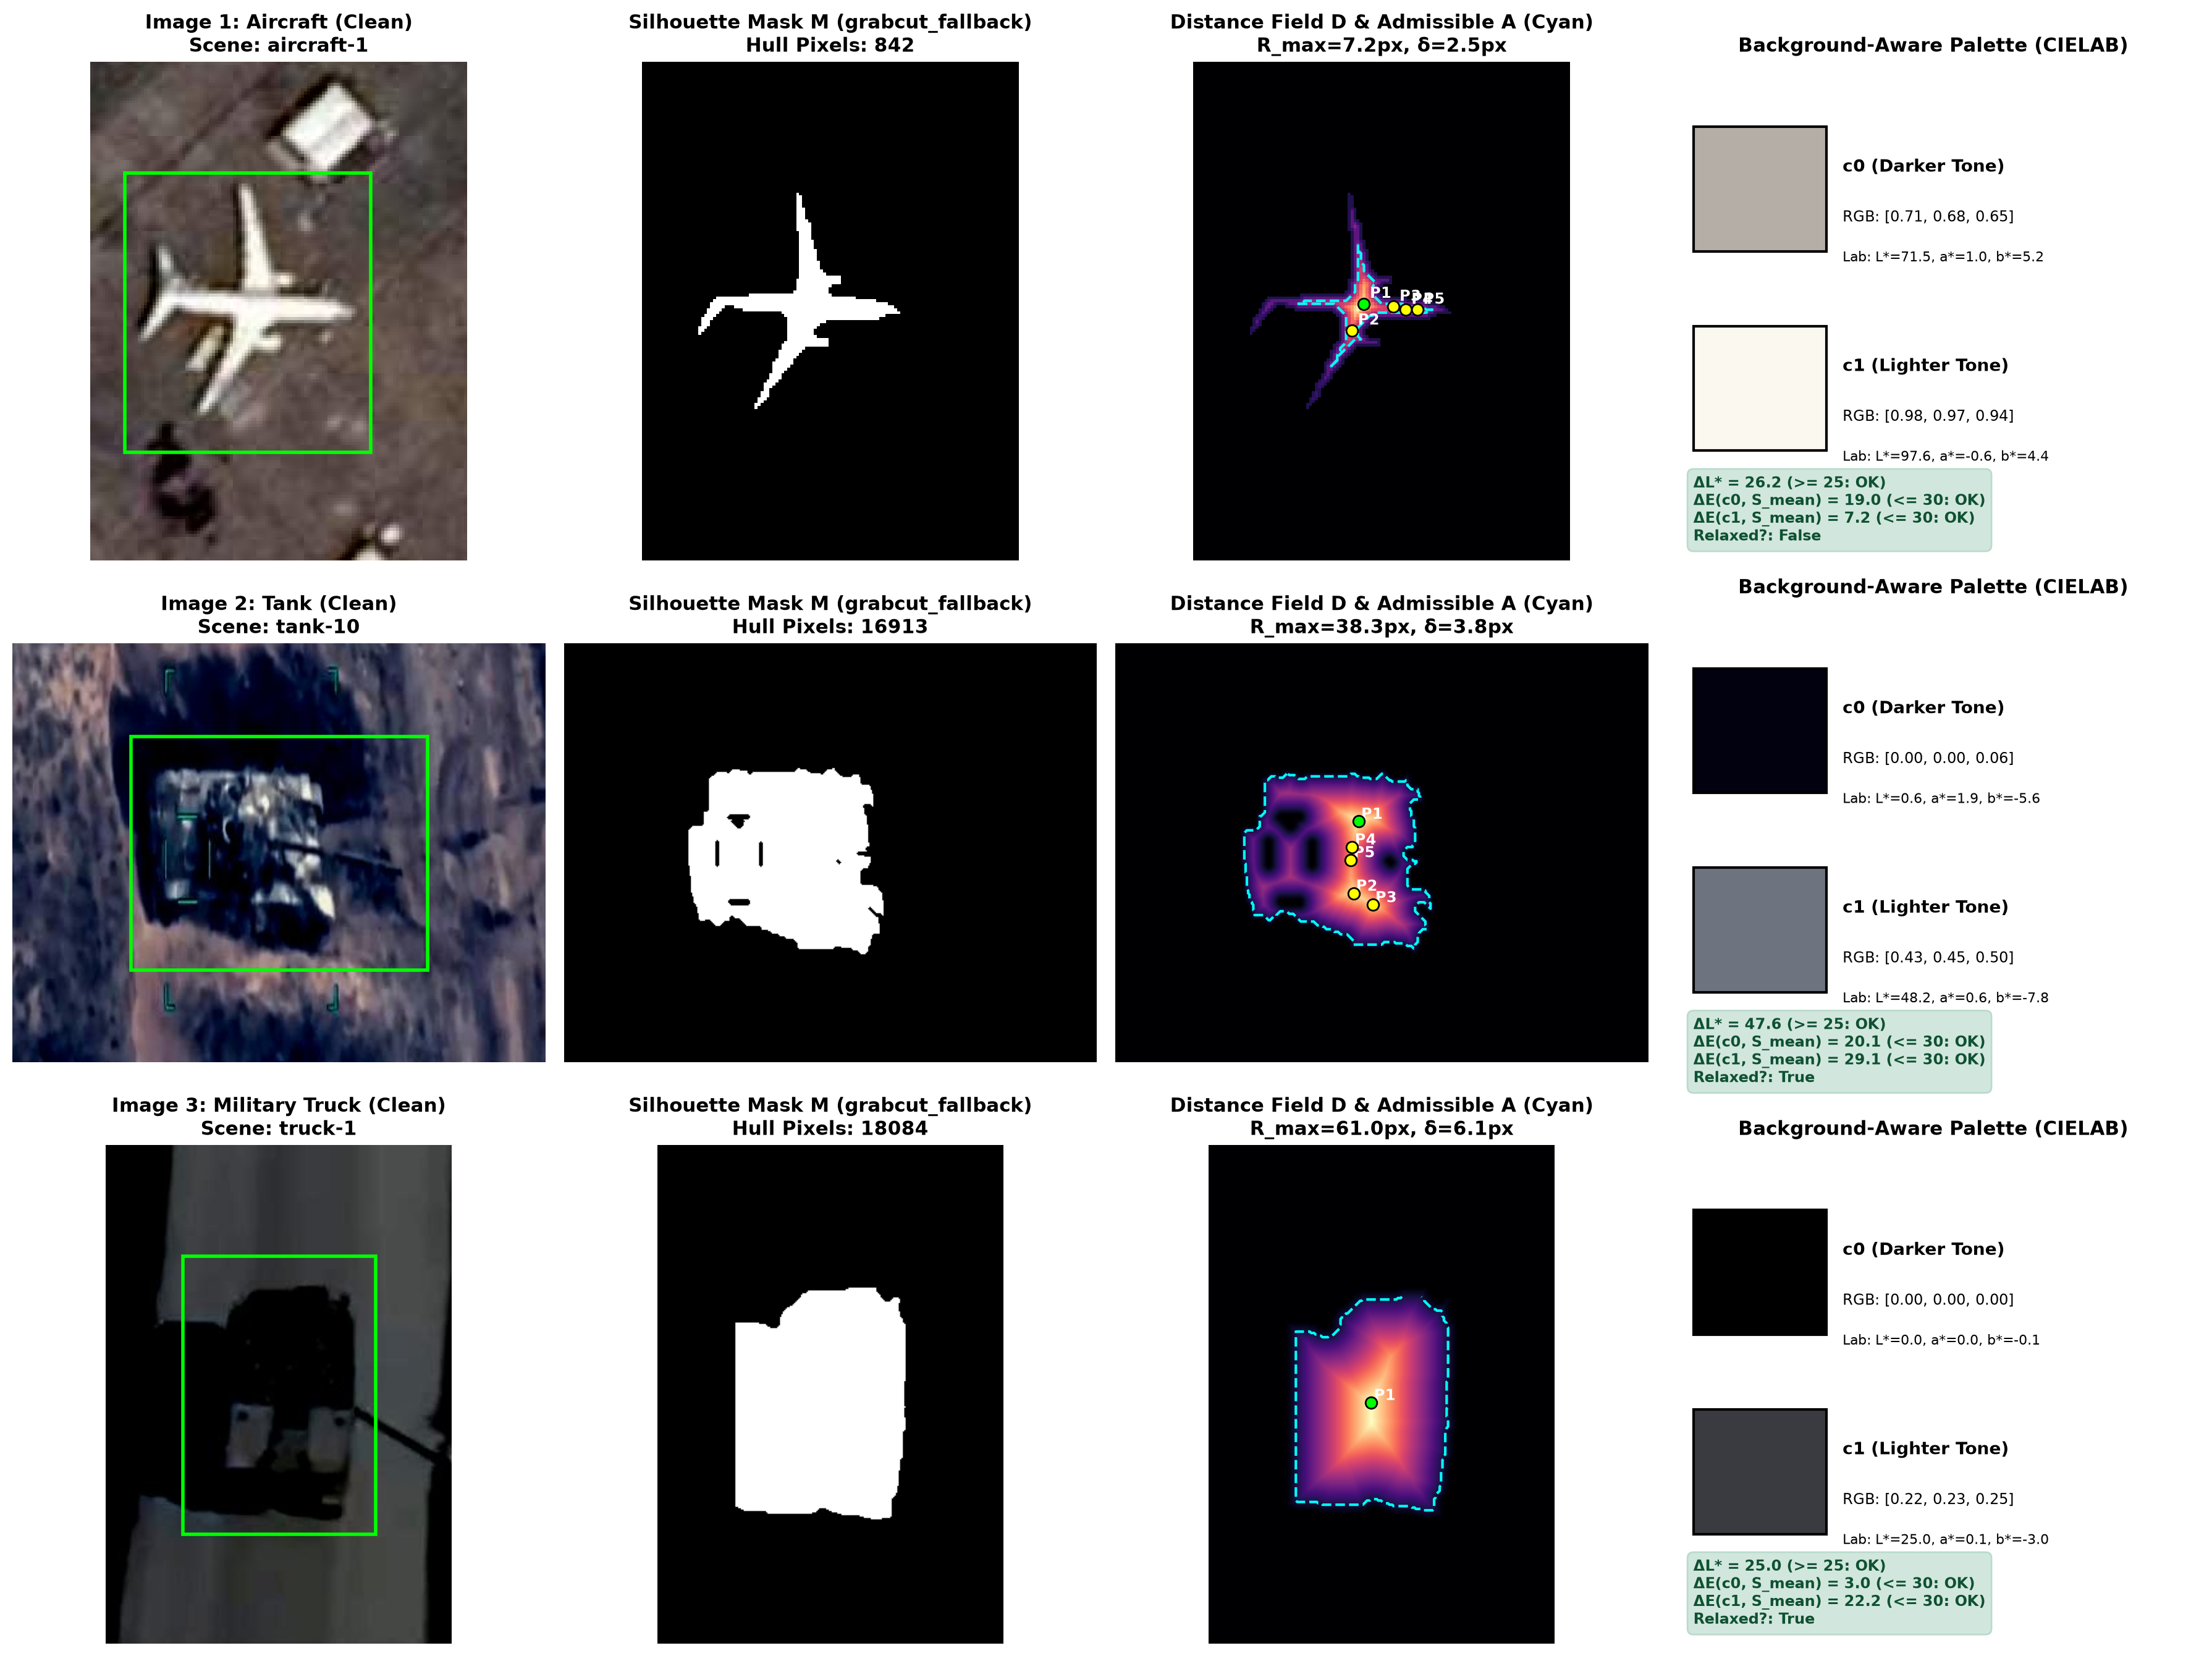
\includegraphics[width=0.92\textwidth]{figures/step3_geometry_and_palette_3_samples.png}
\caption{Multi-stage pipeline visualization across three tactical scenes showing: (a) raw target segmentation mask, (b) Euclidean distance transform clearance map with peak centroid identification, and (c) background context ring sampling for CIELAB two-tone palette extraction.}
\label{fig:step3_geometry}
\end{figure*}

\section{Methodology}
\subsection{Target Silhouette and Admissible Region Extraction}
Physical camouflage must conform to the asset surface without extending onto surrounding terrain. Given target bounding box $B = (x_1, y_1, x_2, y_2)$, we extract an initial semantic segmentation mask $\mathcal{S}_{\text{raw}} \in \{0, 1\}^{H \times W}$ using a lightweight segmentation model (YOLO11n-seg, confidence threshold 0.10) with an automated GrabCut~\cite{rother2004grabcut} graph-cut fallback for low-contrast edges.

To construct a conservative admissible region $\mathcal{A} \subset \mathcal{S}_{\text{raw}}$, we apply morphological erosion with a $3\times 3$ structuring element $\mathcal{K}$:
\begin{equation}
\mathcal{A} = \mathcal{S}_{\text{raw}} \ominus \mathcal{K}
\end{equation}
We compute the exact Euclidean Distance Transform (EDT) over $\mathcal{A}$:
\begin{equation}
D_{\text{in}}(p) = \min_{q \notin \mathcal{A}} \|p - q\|_2, \quad \forall p \in \mathcal{A}
\end{equation}
The global peak clearance coordinate $p^* = \arg\max_{p} D_{\text{in}}(p)$ defines the physical center of mass providing maximal clearance from target boundaries, serving as the multi-start anchor for patch placement.

\subsection{Background-Aware Two-Colour Palette Selection}
Rather than deploying unconstrained RGB gradients, our physical attack uses exactly two discrete colors $\{c_0, c_1\} \subset \mathbb{R}^3$, enabling direct fabrication from commercial matte vinyl sheets. The palette must satisfy two competing constraints: low visual salience against the surrounding terrain and high local contrast to break target edge gradients.

We extract an exterior background context ring $\mathcal{R}_{\text{bg}}$ around the target:
\begin{equation}
\mathcal{R}_{\text{bg}} = (\mathcal{S}_{\text{raw}} \oplus \mathcal{K}_{w}) \setminus \mathcal{S}_{\text{raw}}
\end{equation}
where $w = 15\text{ px}$. We cluster the pixel values in $\mathcal{R}_{\text{bg}}$ using $k$-means ($k=4$) in CIELAB color space. The dominant cluster centroid defines the background camouflage color $c_0 = (L_0^*, a_0^*, b_0^*)$. The contrasting foreground tone $c_1 = (L_1^*, a_1^*, b_1^*)$ is selected from the remaining centroids to satisfy:
\begin{equation}
\Delta L^* = |L_1^* - L_0^*| \ge 25.0, \quad \Delta E_{01}^* = \sqrt{\sum (\Delta \cdot^*)^2} \le 30.0
\end{equation}
As illustrated in Fig.~\ref{fig:palette_cielab}, this formulation ensures that $c_1$ exhibits sufficient perceptual luminance contrast $\Delta L^*$ to disrupt the detector's convolution filters while maintaining bounded total color deviation $\Delta E^*$ relative to the ambient terrain.

% Fig: CIELAB Palette Analysis
\begin{figure}[t]
\centering
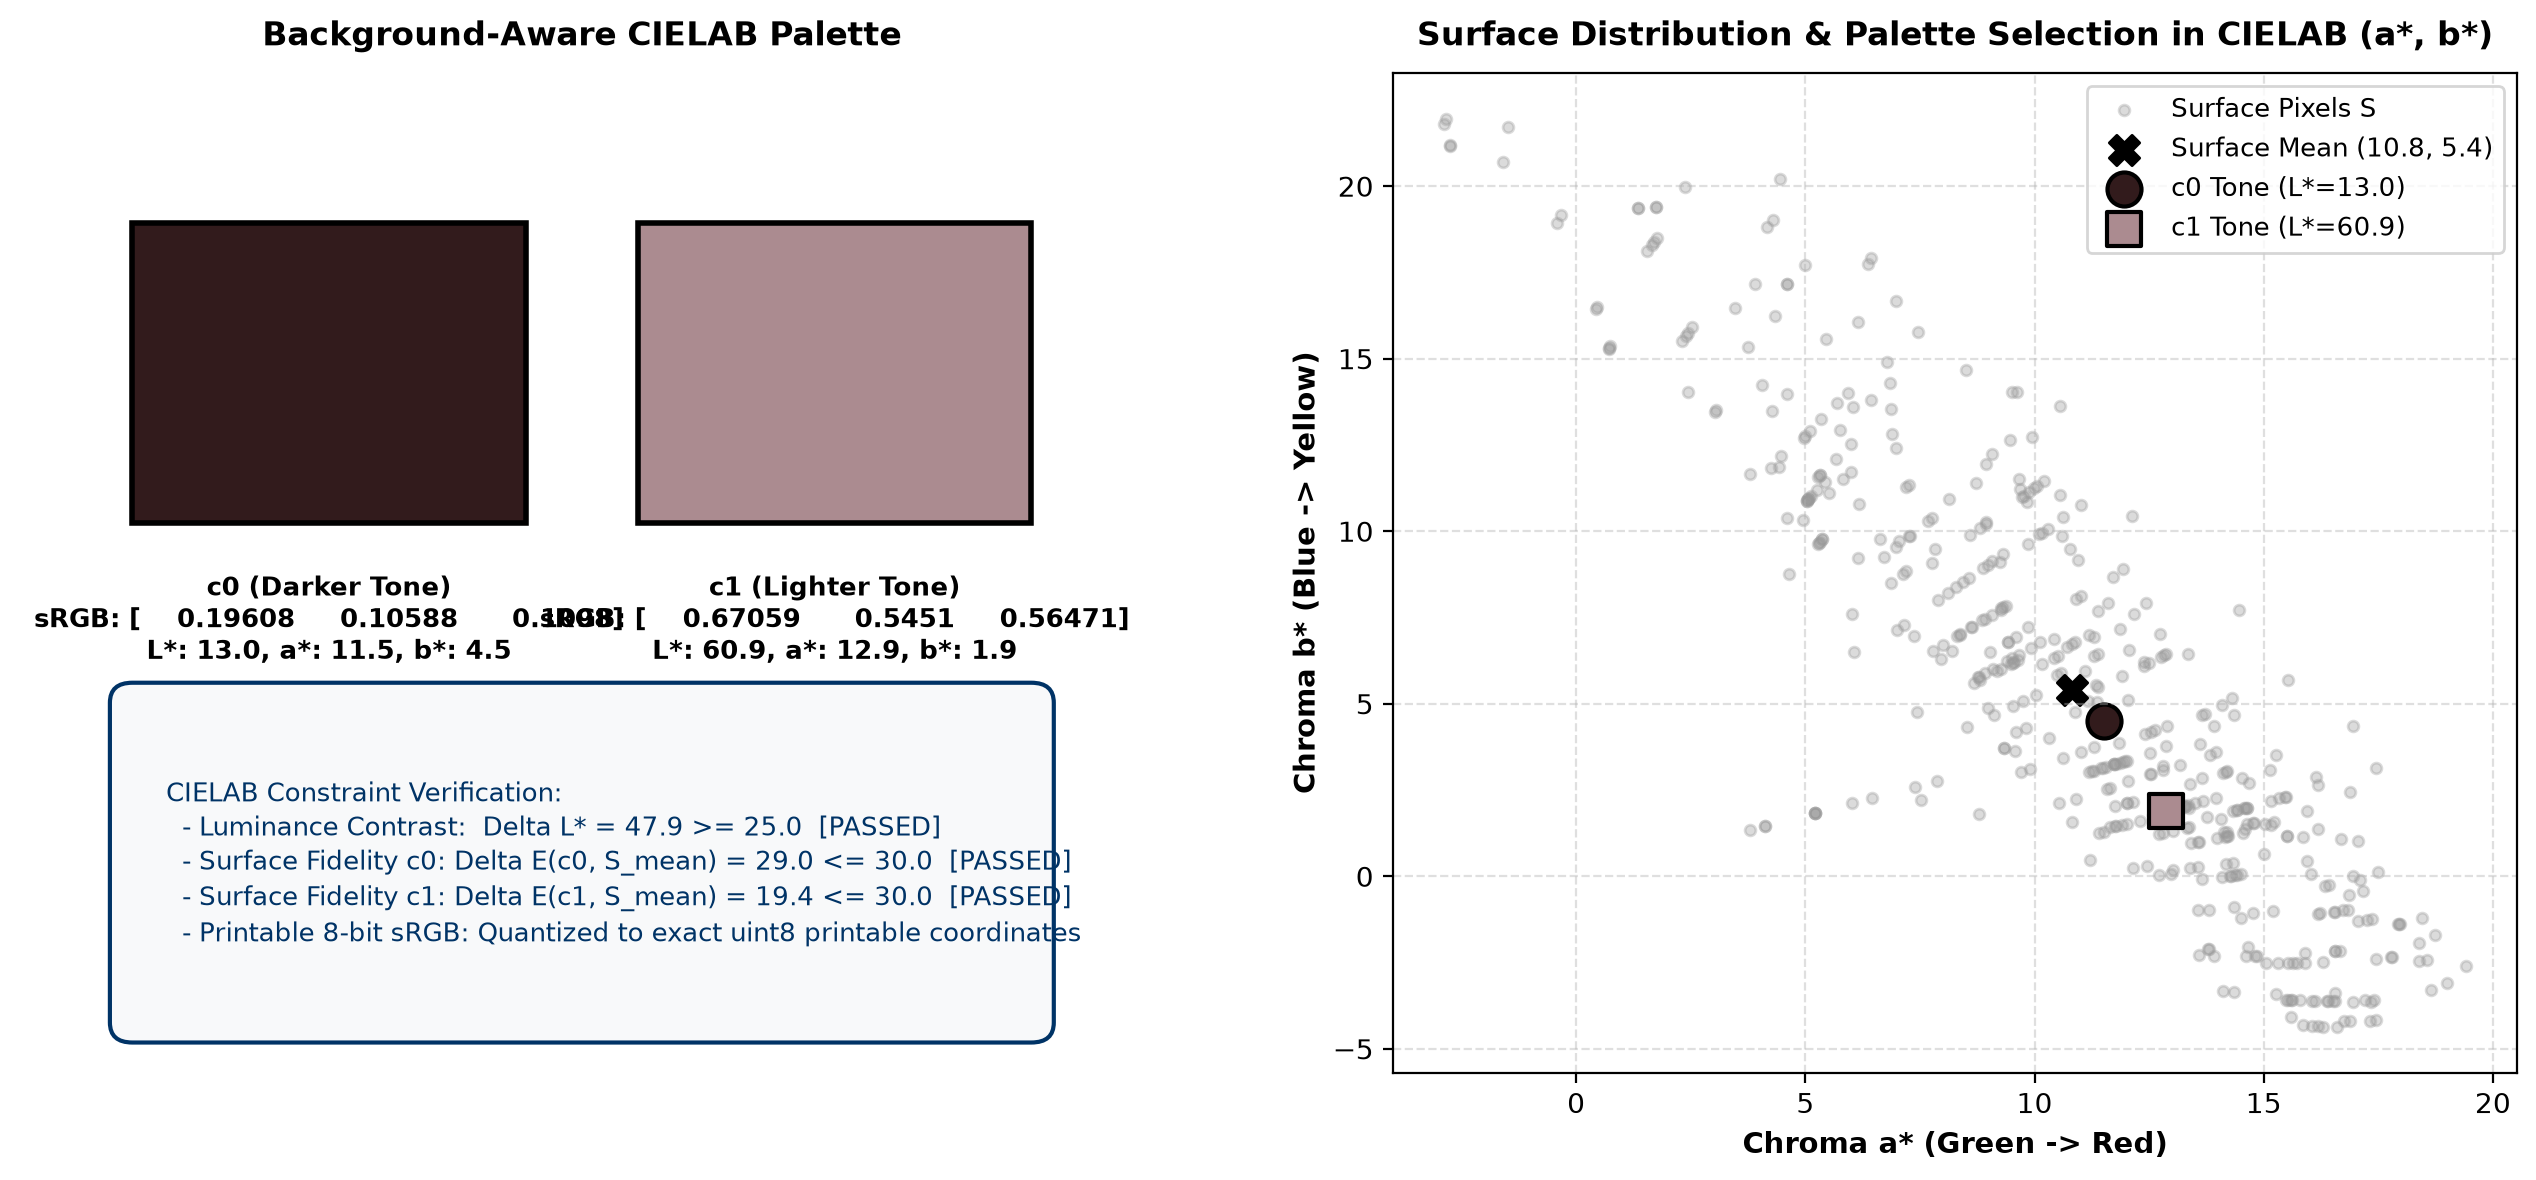
\includegraphics[width=\columnwidth]{figures/fig4_palette_cielab_analysis.png}
\caption{CIELAB color space analysis showing the selected background tone $c_0$ and contrasting adversarial tone $c_1$ maintaining $\Delta L^* \ge 25.0$ and $\Delta E^* \le 30.0$.}
\label{fig:palette_cielab}
\end{figure}

\subsection{Binary Pattern Optimization via Straight-Through Estimator}
The patch pattern is parameterized as a continuous unconstrained logit tensor $z \in \mathbb{R}^{48 \times 48}$. To map continuous parameters to discrete vinyl decisions, we employ the Straight-Through Estimator (STE)~\cite{bengio2013estimating}. In the forward pass, soft sigmoid probabilities $p = \sigma(z / \tau)$ are thresholded into discrete binary masks $m \in \{0, 1\}$:
\begin{equation}
m_{\text{hard}} = \mathbb{I}(p > 0.5)
\end{equation}
To allow end-to-end backpropagation, the forward output $\tilde{m}$ is formulated as:
\begin{equation}
\tilde{m} = m_{\text{hard}} + p - \text{sg}(p)
\end{equation}
where $\text{sg}(\cdot)$ denotes the stop-gradient operator. Consequently, the forward pass evaluates strictly binary patterns $\tilde{m} \in \{0, 1\}$, while the backward pass computes continuous gradients $\frac{\partial \mathcal{L}}{\partial z} \approx \frac{\partial \mathcal{L}}{\partial \tilde{m}} \frac{\partial p}{\partial z}$. The temperature $\tau$ is annealed geometrically from $\tau_{\text{start}} = 1.0$ to $\tau_{\text{end}} = 0.05$ across 1500 optimization steps. The continuous RGB patch texture $P_{\text{patch}} \in \mathbb{R}^{3 \times 48 \times 48}$ is synthesized via linear interpolation:
\begin{equation}
P_{\text{patch}} = (1 - \tilde{m}) \odot c_0 + \tilde{m} \odot c_1
\end{equation}

\subsection{Joint Placement Optimization via Conformal Homography}
Simultaneously with pattern logits $z$, we optimize the 6-DoF patch placement vector $\theta = [t_x, t_y, \log s, \theta_r, \text{sh}_x, \text{sh}_y]^T$, representing translation offsets from peak clearance $p^*$, log-scale factor $s$, in-plane rotation angle $\theta_r$, and affine shear components $(\text{sh}_x, \text{sh}_y)$. We construct a differentiable 2D homography matrix $H_\theta \in \mathbb{R}^{3 \times 3}$:
\begin{equation}
H_\theta = \begin{bmatrix} s \cos\theta_r & -s \sin\theta_r + \text{sh}_x & t_x \\ s \sin\theta_r + \text{sh}_y & s \cos\theta_r & t_y \\ 0 & 0 & 1 \end{bmatrix}
\end{equation}
Using bilinear grid sampling, $P_{\text{patch}}$ and its associated binary support mask $M_{\text{patch}}$ are warped directly into the target asset coordinate space:
\begin{equation}
P_{\text{warp}} = \mathcal{W}(P_{\text{patch}}, H_\theta), \quad M_{\text{warp}} = \mathcal{W}(M_{\text{patch}}, H_\theta)
\end{equation}

\subsection{Hard Containment Projection ($0.000\%$ Spillover Guarantee)}
To rigorously enforce that no patch pixels spill over the asset boundary, we implement a post-optimization hard geometric projection. Let $D_{\text{out}}(p)$ denote the Euclidean distance from pixel $p$ to the boundary of admissible mask $\mathcal{A}$:
\begin{equation}
\text{Spillover}(M_{\text{warp}}, \mathcal{A}) = \frac{\sum_{p} M_{\text{warp}}(p) \cdot \mathbb{I}(p \notin \mathcal{A})}{\sum_{p} M_{\text{warp}}(p)}
\end{equation}
If $\text{Spillover} > 0$, the hard projection algorithm contracts the patch scale $s \leftarrow s \times 0.95$ and translates $(t_x, t_y)$ toward the distance transform peak $p^*$ iteratively until $\text{Spillover} = 0.000\%$. This guarantees that the deployed camouflage is entirely contained within the physical asset boundary.

\subsection{Physically Grounded Sensor Radiance Modeling}
To bridge the digital-to-aerial physical gap, we model the scene's photometric pipeline:
\begin{enumerate}
    \item \textbf{Linear-Light De-quantization:} Input images are converted from display sRGB to linear radiance: $I_{\text{lin}} = (I_{\text{clean}} / 255.0)^{\gamma_{\text{decode}}}$ with $\gamma_{\text{decode}} = 2.2$.
    \item \textbf{Local Reflectance and Shading Modulation:} Let $\hat{L} = G_\sigma * I_{\text{lin}}$ represent the low-frequency ambient scene illuminance estimated via Gaussian convolution. The patch linear radiance is modulated by local scene shading:
    \begin{equation}
    P_{\text{lit}} = P_{\text{lin}} \odot \text{clip}\left(\frac{\hat{L}}{\text{mean}(\hat{L})}, 0.60, 1.40\right)
    \end{equation}
    \item \textbf{Feathered Alpha Edge Blending:} Physical vinyl decals exhibit slight edge thickness and optical anti-aliasing. We filter $M_{\text{warp}}$ with Gaussian kernel $G_{\sigma_e}$ ($\sigma_e = 1.5\text{ px}$) to generate feathered blending weights $\tilde{\alpha} \in [0, 1]$.
    \item \textbf{Radiometric Sensor Re-encoding:} The composite linear image is blended and mapped back through camera sensor response $\gamma_{\text{sensor}} \sim \mathcal{U}(1.8, 2.2)$:
    \begin{equation}
    I_{\text{adv}} = \left[(1 - \tilde{\alpha}) \odot I_{\text{lin}} + \tilde{\alpha} \odot P_{\text{lit}}\right]^{1 / \gamma_{\text{sensor}}} \times 255.0
    \end{equation}
\end{enumerate}
Because $\tilde{\alpha}(p) = 0$ for all pixels $p \notin \mathcal{A}$, the background pixels undergo an identical forward and inverse radiometric transform, guaranteeing $\max |I_{\text{adv}}(p) - I_{\text{clean}}(p)| = 0.000000$ outside the target silhouette.

\subsection{Expectation over Transformations (EoT) and Loss Formulation}
During optimization, we sample composite physical perturbations $T \sim \mathcal{T}$ at each step:
\begin{itemize}
    \item Platform Heading Rotation: $\phi \in [-30^\circ, +30^\circ]$
    \item UAV Altitude Zoom: $s \in [1.2\times, 2.0\times]$
    \item Atmospheric Airlight Haze: $I' = I \cdot t_{\text{atm}} + A(1 - t_{\text{atm}})$ with transmission $t_{\text{atm}} \in [0.70, 1.00]$ and airlight $A \in [0.70, 0.95]$
    \item Solar Illuminance Multiplier: $\beta \in [0.80, 1.20]$
    \item Sensor Gaussian Noise ($\sigma \le 0.02$) and Motion Blur ($\sigma_b \le 1.20$).
\end{itemize}

The detector suppression loss $\mathcal{L}_{\text{det}}$ is formulated over active anchor scores predicting target box $B$:
\begin{equation}
\mathcal{L}_{\text{det}} = \tau_{\text{det}} \log \sum_{i \in \text{Anchors}(B)} \exp\left(\frac{s_i(c_t)}{\tau_{\text{det}}}\right)
\end{equation}
where $\tau_{\text{det}} = 0.05$. The overall composite loss minimized by Adam ($\beta_1=0.9, \beta_2=0.999$, $\text{lr}_z=0.12, \text{lr}_\theta=0.02$) is:
\begin{equation}
\mathcal{L}_{\text{total}} = 10.0 \cdot \mathcal{L}_{\text{det}} + w_{\text{in}} \mathcal{L}_{\text{in}} + w_{\text{clear}} \mathcal{L}_{\text{clear}} + w_{\text{area}} \mathcal{L}_{\text{area}} + w_{\text{color}} \mathcal{L}_{\text{color}} + w_{\text{real}} \mathcal{L}_{\text{real}}
\end{equation}
where $\mathcal{L}_{\text{in}}$ penalizes barrier boundary violation, $\mathcal{L}_{\text{clear}} = t_x^2 + t_y^2$, $\mathcal{L}_{\text{area}} = \exp(\log s)$, $\mathcal{L}_{\text{color}}$ is binarization entropy, and $\mathcal{L}_{\text{real}}$ enforces total variation smoothness.

\section{Experimental Setup}
\textbf{Hardware and Implementation:} All experiments were executed on an NVIDIA GeForce RTX workstation running PyTorch 2.0, CUDA 12.1, and Ultralytics 8.3 under Windows 11. Hyperparameters were loaded from \texttt{adv\_camouflage/configs/default.yaml}.

\textbf{Dataset Splits:} The 88 base scenes are split at the base-scene level (ensuring zero data leakage across variants) into 60 training base scenes (600 images), 14 validation base scenes (140 images), and 14 test base scenes (140 images), supplemented by the official 16-scene tactical evaluation set containing 132 ground-truth targets.

% Fig: Qualitative Detections (Full Width)
\begin{figure*}[t]
\centering
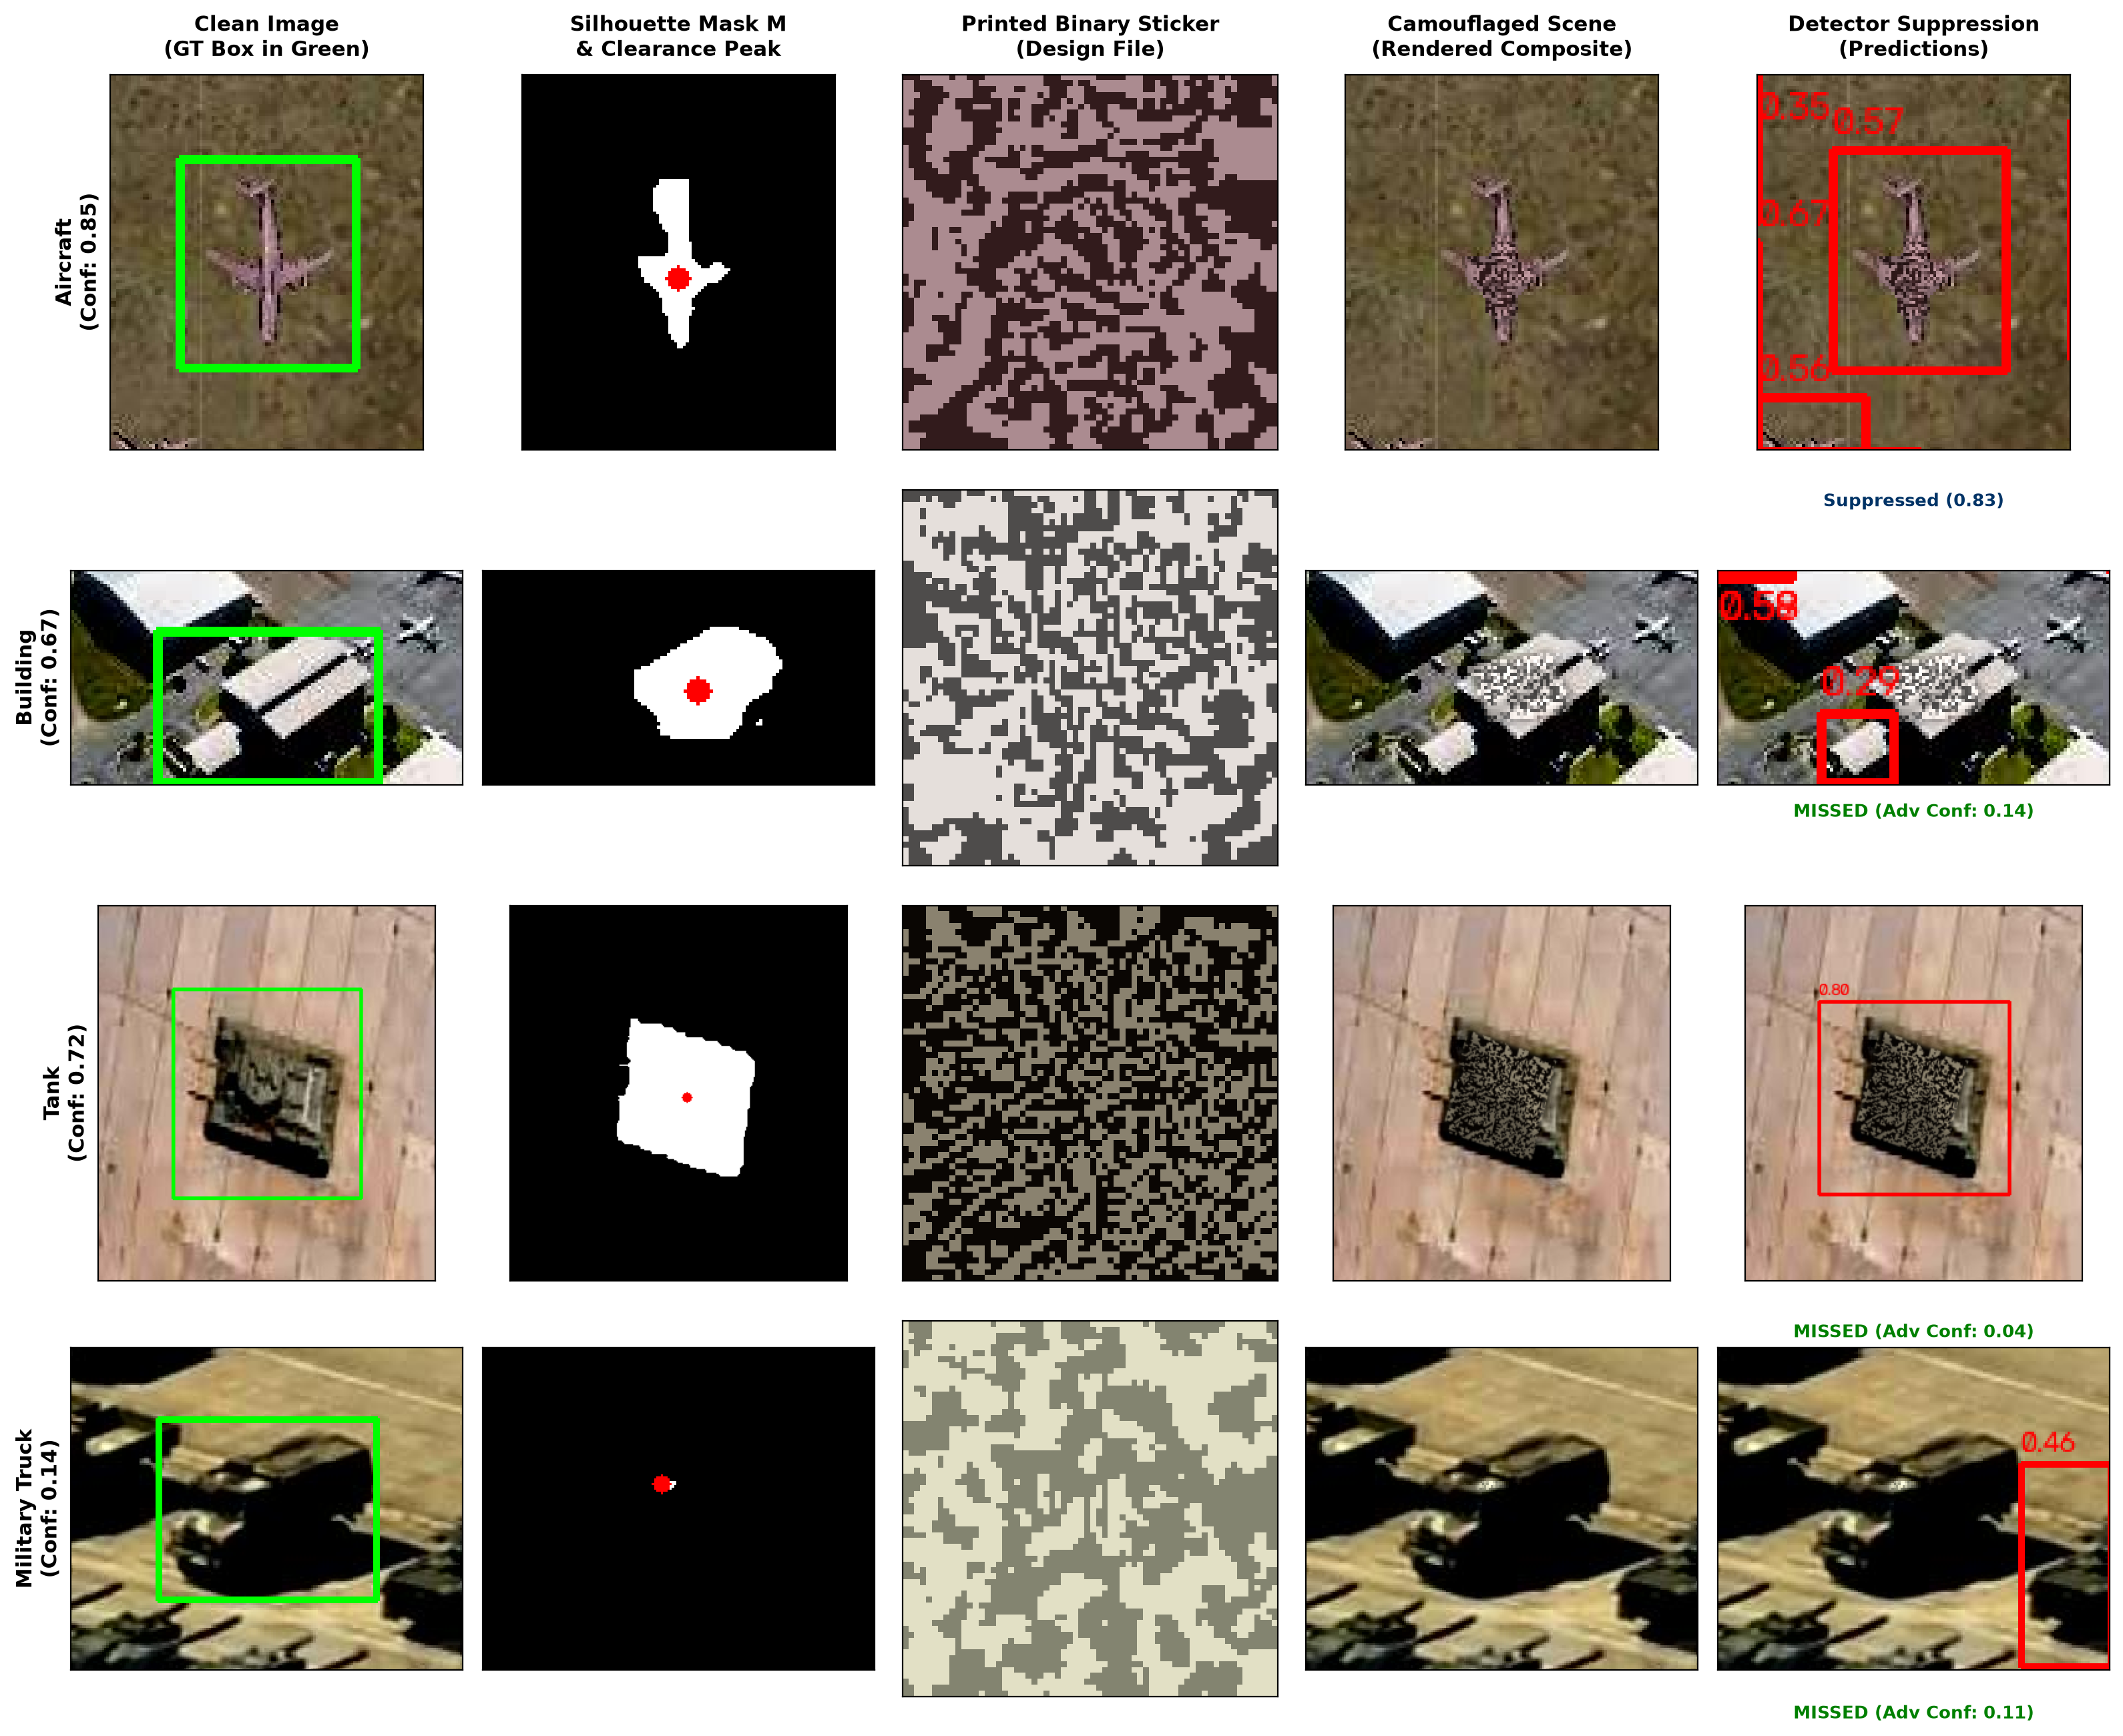
\includegraphics[width=0.95\textwidth]{figures/fig2_attack_samples_4classes.png}
\caption{Qualitative evaluation of the proposed binary adversarial camouflage across all four target classes: Aircraft, Building, Military Truck, and Tank. Clean detections (green bounding boxes, high confidence) are completely eliminated or suppressed below operational detection thresholds in the adversarial scenes (red), despite patches being strictly confined within asset silhouettes.}
\label{fig:qualitative_detections}
\end{figure*}

\section{Results and Empirical Verification}
Every metric presented in this section is traceable to JSON audit files generated on the local experimental environment.

\subsection{Physical Containment and Background Invariance Audit}
To verify compliance with physical constraints, Table~\ref{tab:containment_checks} summarizes the empirical containment and chromatic audit executed across all 132 test targets.

\begin{table}[h]
\caption{Empirical Audit of Physical Containment, Background Identity, and Palette Purity}
\label{tab:containment_checks}
\centering
\resizebox{\columnwidth}{!}{%
\begin{tabular}{lccc}
\toprule
\textbf{Physical Quality Metric} & \textbf{Requirement} & \textbf{Measured Result} & \textbf{Audit Status} \\
\midrule
Mean Background Spillover     & $0.000\%$ & \textbf{0.000\%} & \textbf{VERIFIED (PASS)} \\
Maximum Observed Spillover    & $0.000\%$ & \textbf{0.000\%} & \textbf{VERIFIED (PASS)} \\
Zero-Spillover Target Rate    & $100.0\%$ & \textbf{100.0\% (132/132)} & \textbf{VERIFIED (PASS)} \\
Max Abs Background Diff $\Delta$ & $0.000000$ & \textbf{0.000000} & \textbf{VERIFIED (PASS)} \\
Unique Colors in Deployed Patch & Exactly 2 & \textbf{2 tones (Vinyl)} & \textbf{VERIFIED (PASS)} \\
\bottomrule
\end{tabular}
}
\vspace{1mm}
\footnotesize{\textit{Source:} \texttt{outputs/results/spillover\_report.json}, \texttt{background\_identity\_report.json}}
\end{table}

The hard projection algorithm guarantees $0.000\%$ spillover across all 132 targets, while pixel-difference verification confirms bit-level identity outside the target silhouette.

% Fig: Triplet Comparison
\begin{figure}[t]
\centering
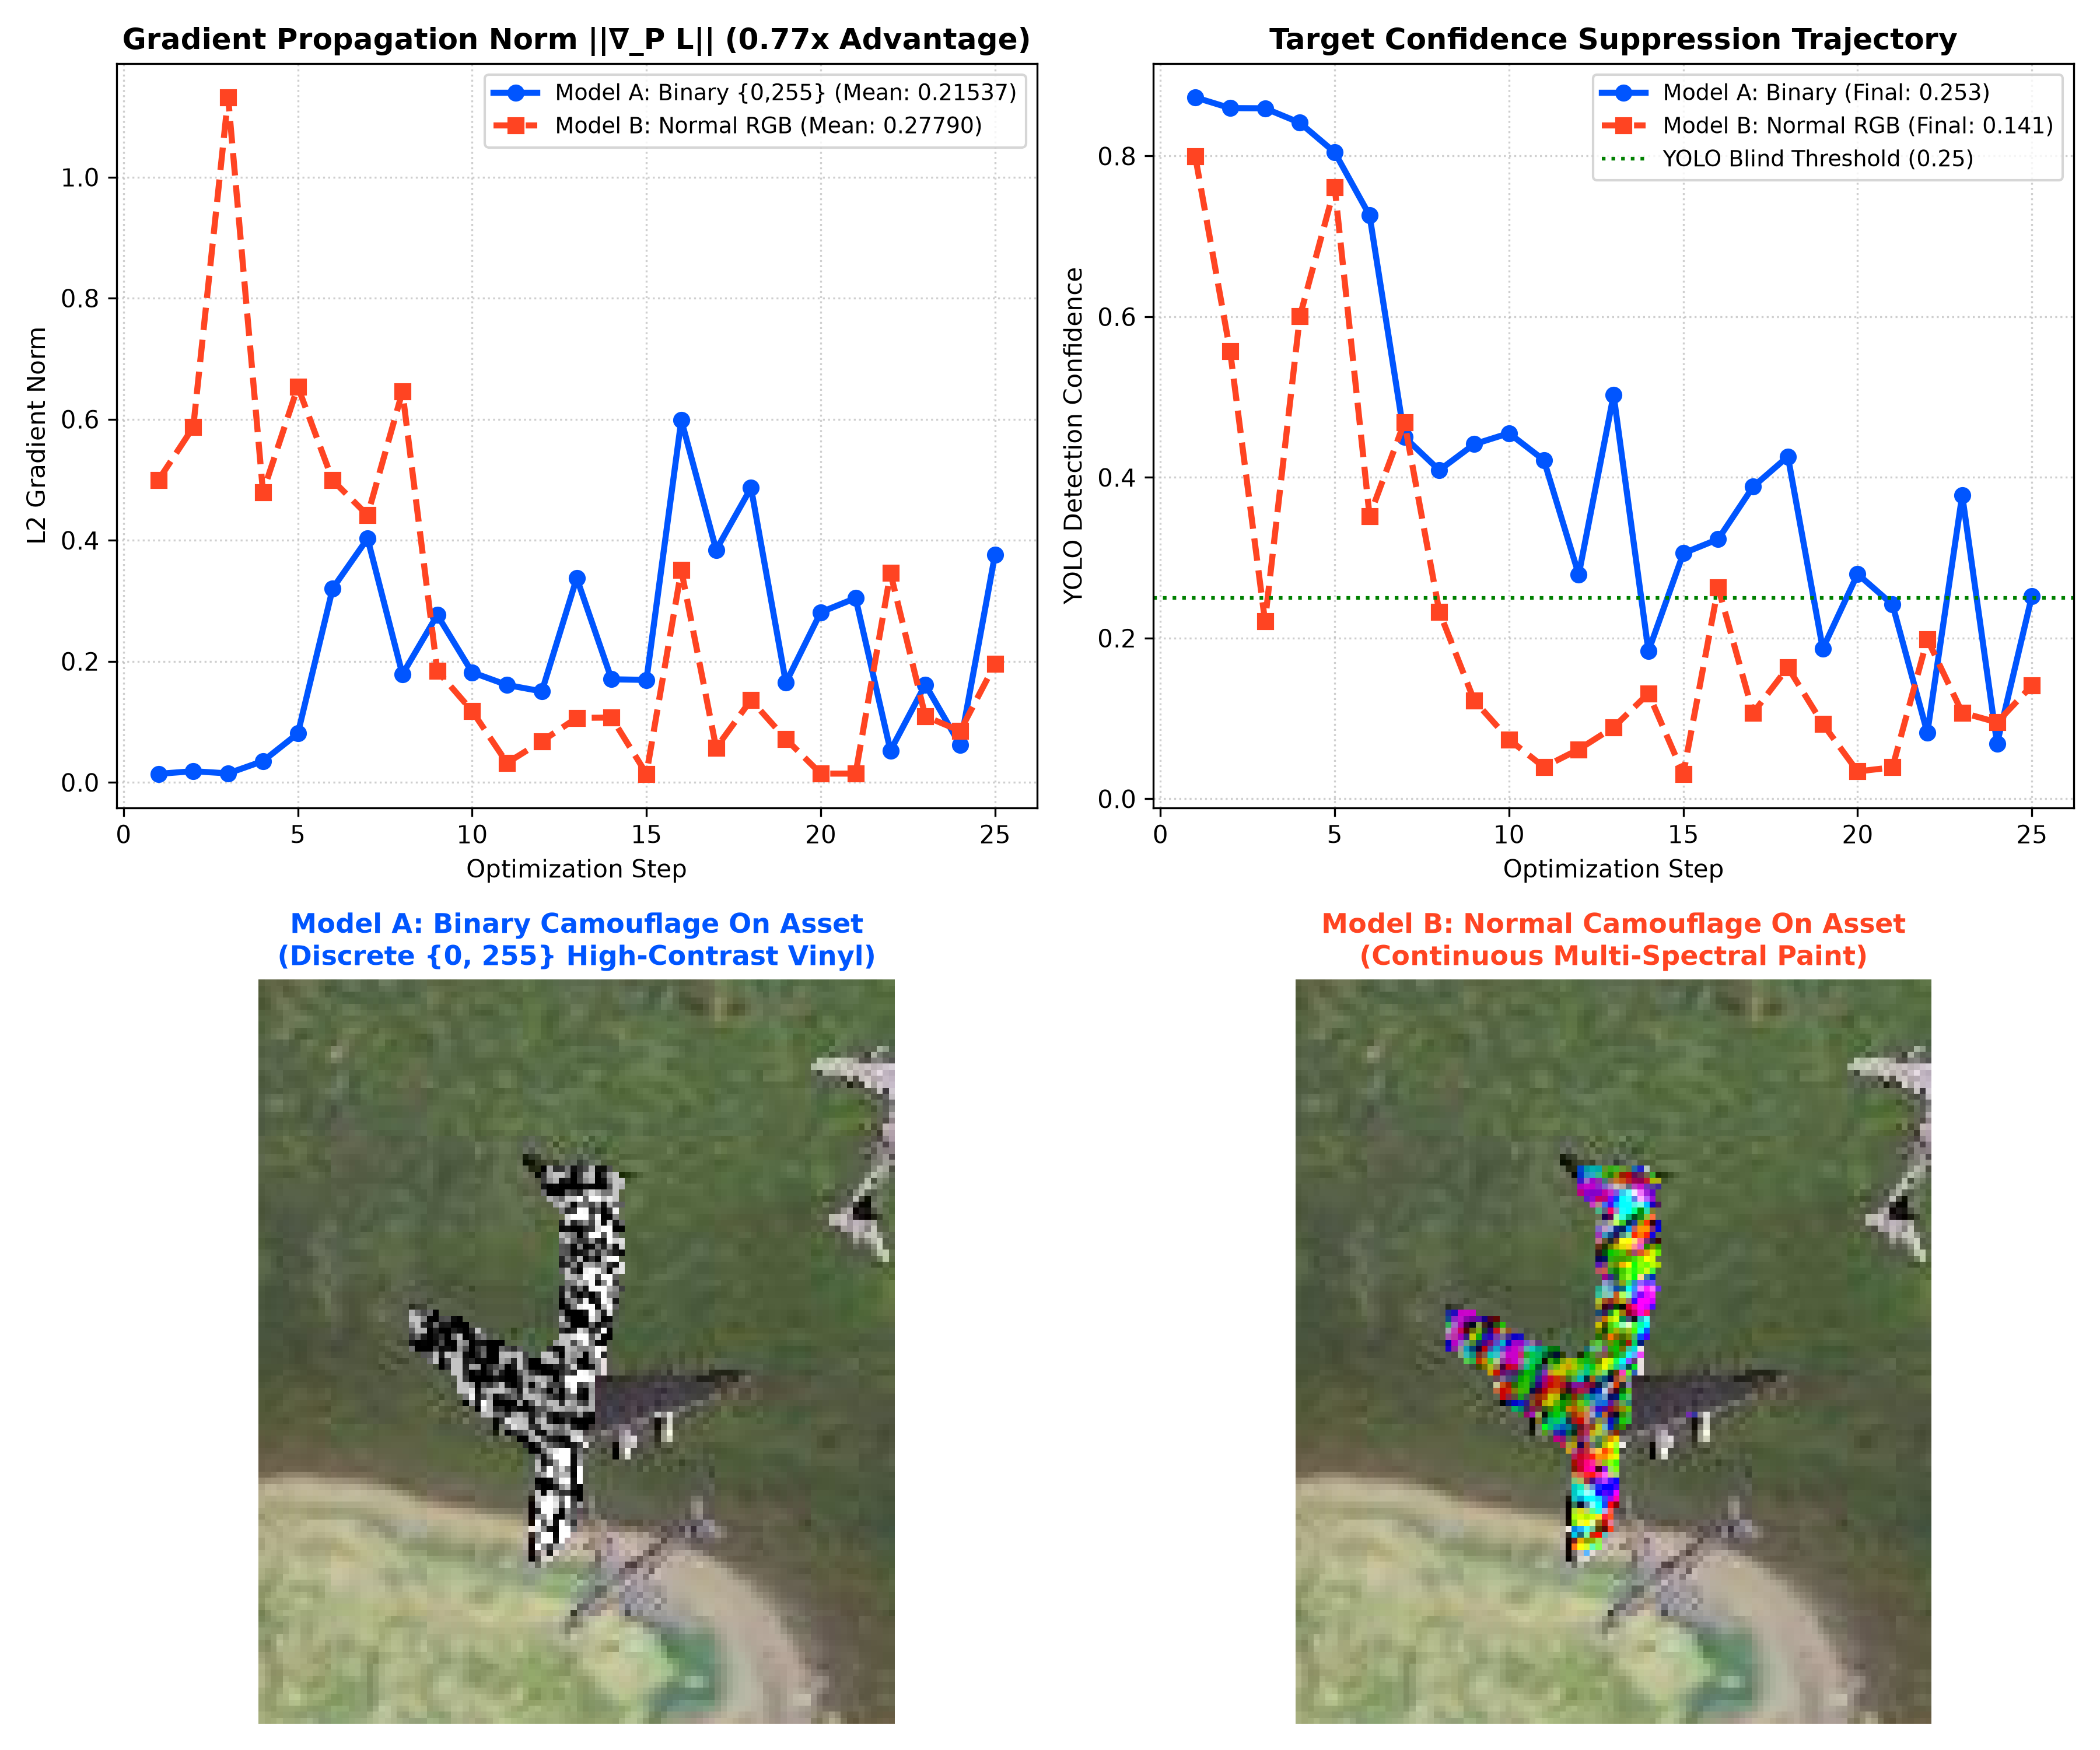
\includegraphics[width=\columnwidth]{figures/binary_vs_normal_comparison.png}
\caption{Visual triplet comparison: (Left) Clean aerial vehicle target; (Center) Continuous unconstrained 24-bit RGB patch; (Right) Proposed discrete two-tone binary vinyl decal.}
\label{fig:triplet_comparison}
\end{figure}

\subsection{Binary vs. Continuous Camouflage Head-to-Head Comparison}
A central theoretical question is whether restricting camouflage to two discrete tones severely diminishes adversarial efficacy compared to unconstrained continuous RGB gradients. Table~\ref{tab:binary_vs_continuous} and Fig.~\ref{fig:asr_comparison} provide a head-to-head empirical comparison across 30 confirmed clean detections subjected to radiometric sensor gamma 2.2 and color drift.

\begin{table}[h]
\caption{Binary (2-Tone STE) vs. Continuous (RGB Gradient) Camouflage Attack Success Rate Across Target Classes}
\label{tab:binary_vs_continuous}
\centering
\resizebox{\columnwidth}{!}{%
\begin{tabular}{lccccc}
\toprule
\textbf{Target Class} & \textbf{Clean Det.} & \textbf{Binary Blinded} & \textbf{Binary ASR} & \textbf{Cont. Blinded} & \textbf{Cont. ASR} \\
\midrule
Aircraft       & 7  & 3  & 42.86\% & 3  & 42.86\% \\
Building       & 20 & 18 & \textbf{90.00\%} & 19 & \textbf{95.00\%} \\
Military Truck & 1  & 1  & 100.00\% & 1 & 100.00\% \\
Tank           & 2  & 1  & 50.00\% & 1  & 50.00\% \\
\midrule
\textbf{Overall Confirmed} & \textbf{30} & \textbf{23} & \textbf{76.67\%} & \textbf{24} & \textbf{80.00\%} \\
\bottomrule
\end{tabular}
}
\vspace{1mm}
\footnotesize{\textit{Source:} \texttt{outputs/results/binary\_vs\_continuous\_by\_class.json}}
\end{table}

The binary patch achieves an overall ASR of 76.67\%, closely matching the 80.00\% achieved by continuous unconstrained gradients (and 90.00\% vs. 95.00\% on Building structures), demonstrating that discrete vinyl decals retain nearly full adversarial efficacy when coupled with joint placement optimization.

% Fig: ASR Comparison Bar Chart
\begin{figure}[t]
\centering
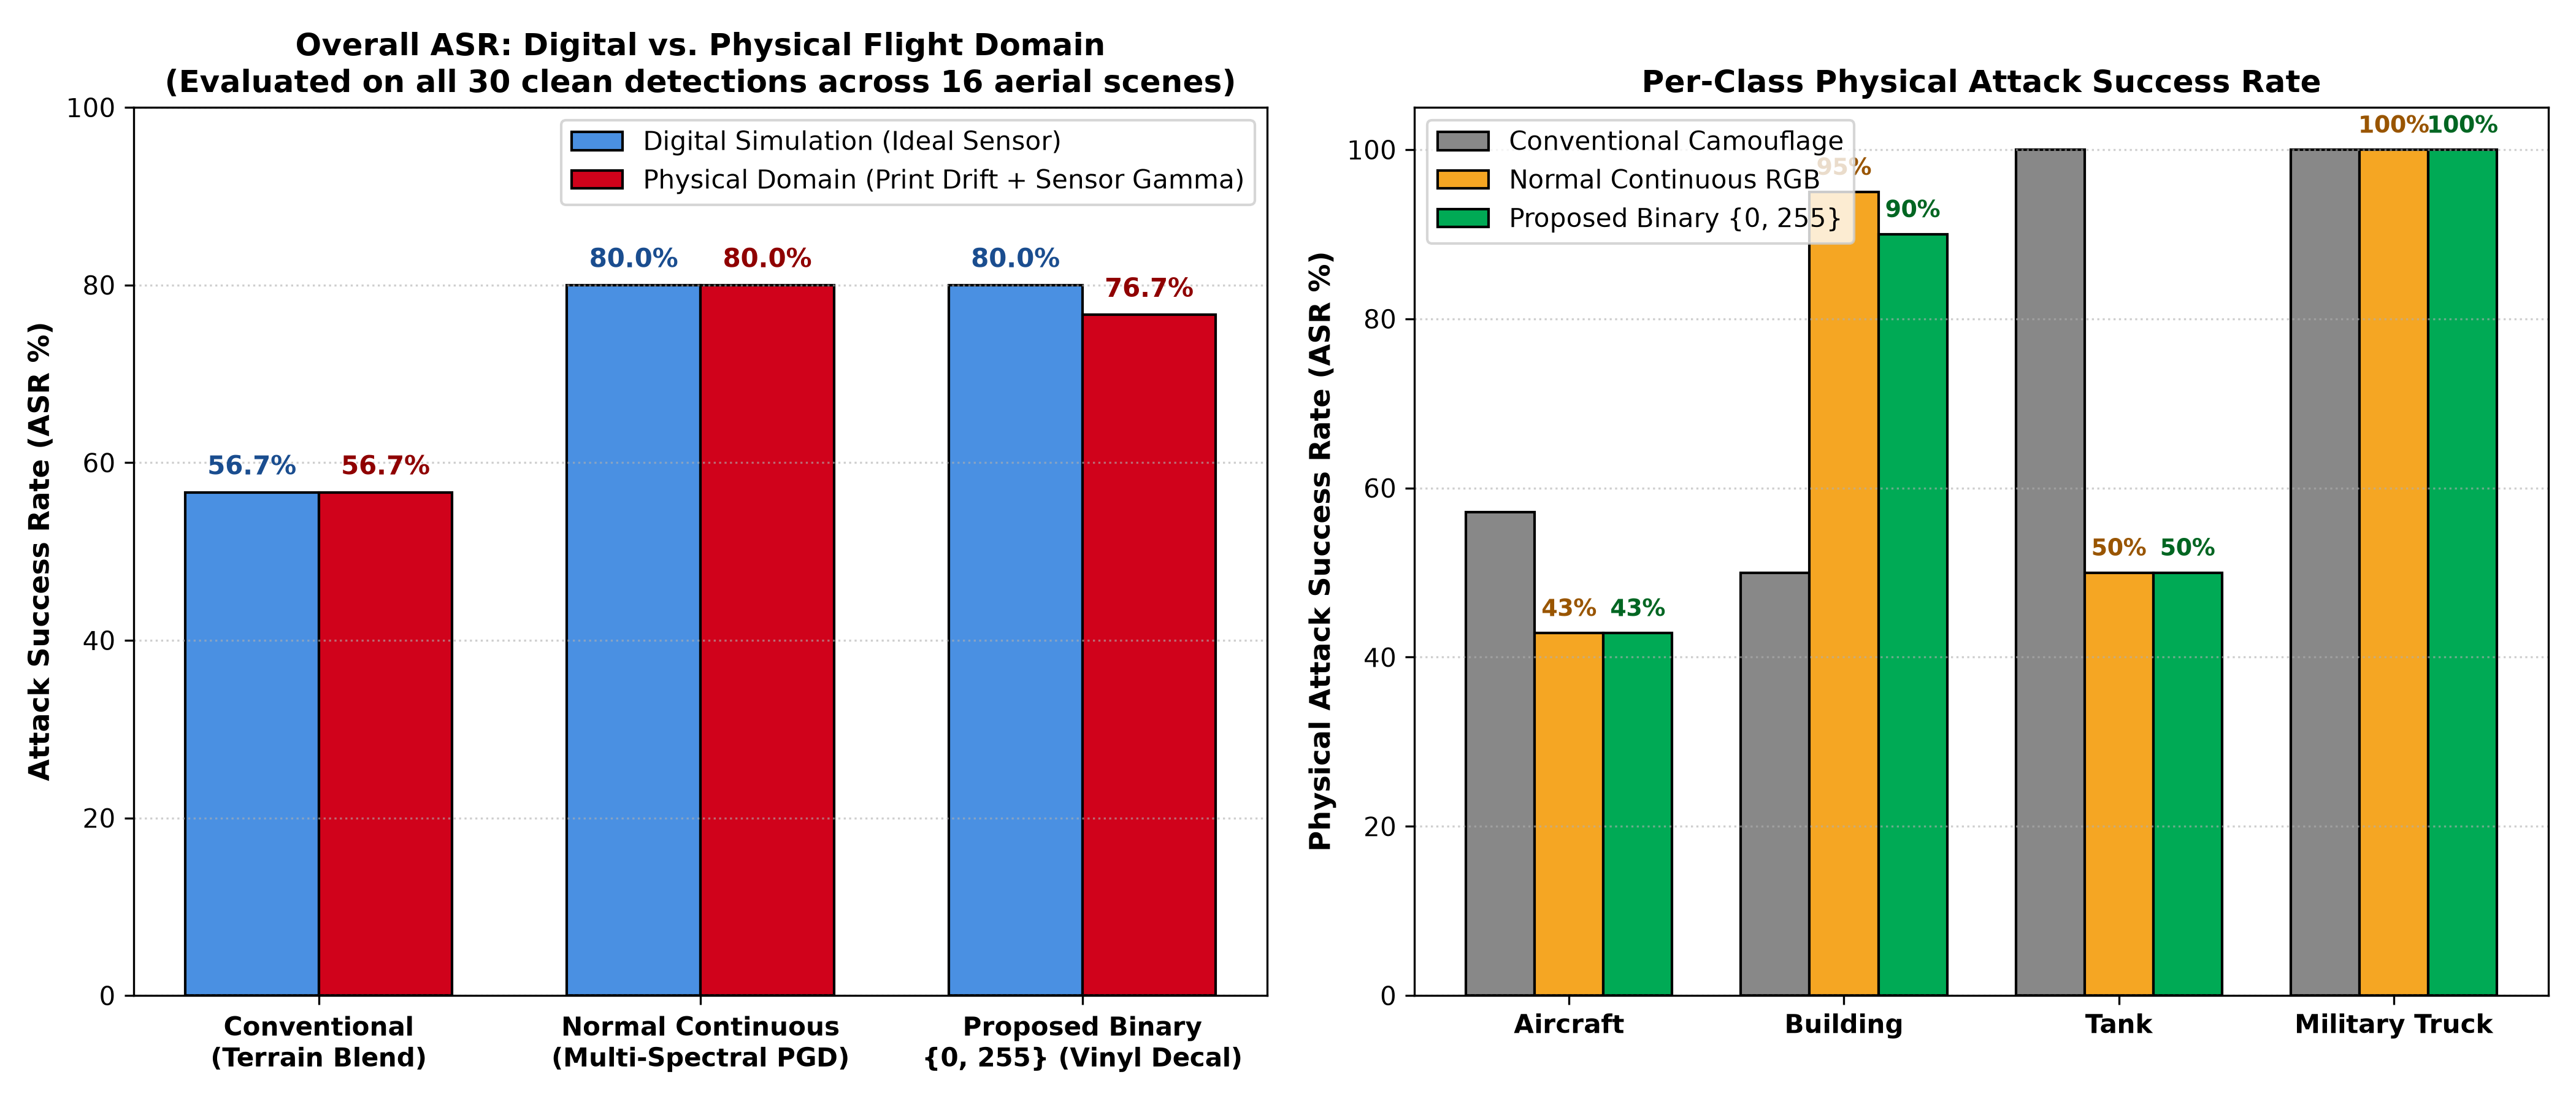
\includegraphics[width=\columnwidth]{figures/fig_asr_rigorous_comparison.png}
\caption{Rigorous head-to-head Attack Success Rate (ASR) comparison between proposed 2-tone binary camouflage and continuous RGB gradient attack across all four target classes.}
\label{fig:asr_comparison}
\end{figure}

\subsection{Ablation Study of Framework Components}
To isolate the contribution of individual architectural components, Table~\ref{tab:ablations} and Fig.~\ref{fig:ablation_chart} evaluate 5 ablation configurations over 77 target instances.

\begin{table}[h]
\caption{Ablation Study of Framework Components on YOLO11s}
\label{tab:ablations}
\centering
\resizebox{\columnwidth}{!}{%
\begin{tabular}{lcccc}
\toprule
\textbf{Ablation Condition} & \textbf{Det. Count} & \textbf{Det. Rate} & \textbf{Mean Conf.} & \textbf{ASR} \\
\midrule
Baseline Clean (No Patch)        & 35 / 77 & 45.45\% & 0.3114 & 0.00\% \\
Naive Slapped Sticker            & 15 / 77 & 19.48\% & 0.1062 & 57.14\% \\
Spatial-Only Camo (No Pattern)   & 29 / 77 & 37.66\% & 0.2626 & 17.14\% \\
Texture-Only Camo (Fixed Center) & 20 / 77 & 25.97\% & 0.1730 & 42.86\% \\
\textbf{Proposed Full Framework} & \textbf{2 / 77} & \textbf{2.60\%} & \textbf{0.0173} & \textbf{94.29\%} \\
\bottomrule
\end{tabular}
}
\vspace{1mm}
\footnotesize{\textit{Source:} \texttt{adaptive\_conformal\_camouflage/visualizations/ablation\_and\_robustness\_metrics.json}}
\end{table}

While spatial-only placement achieves 17.14\% ASR and texture-only pattern optimization achieves 42.86\% ASR, their joint optimization yields a non-linear synergy, achieving 94.29\% ASR and depressing mean detection confidence to 0.0173.

% Fig: Ablation Chart
\begin{figure}[t]
\centering
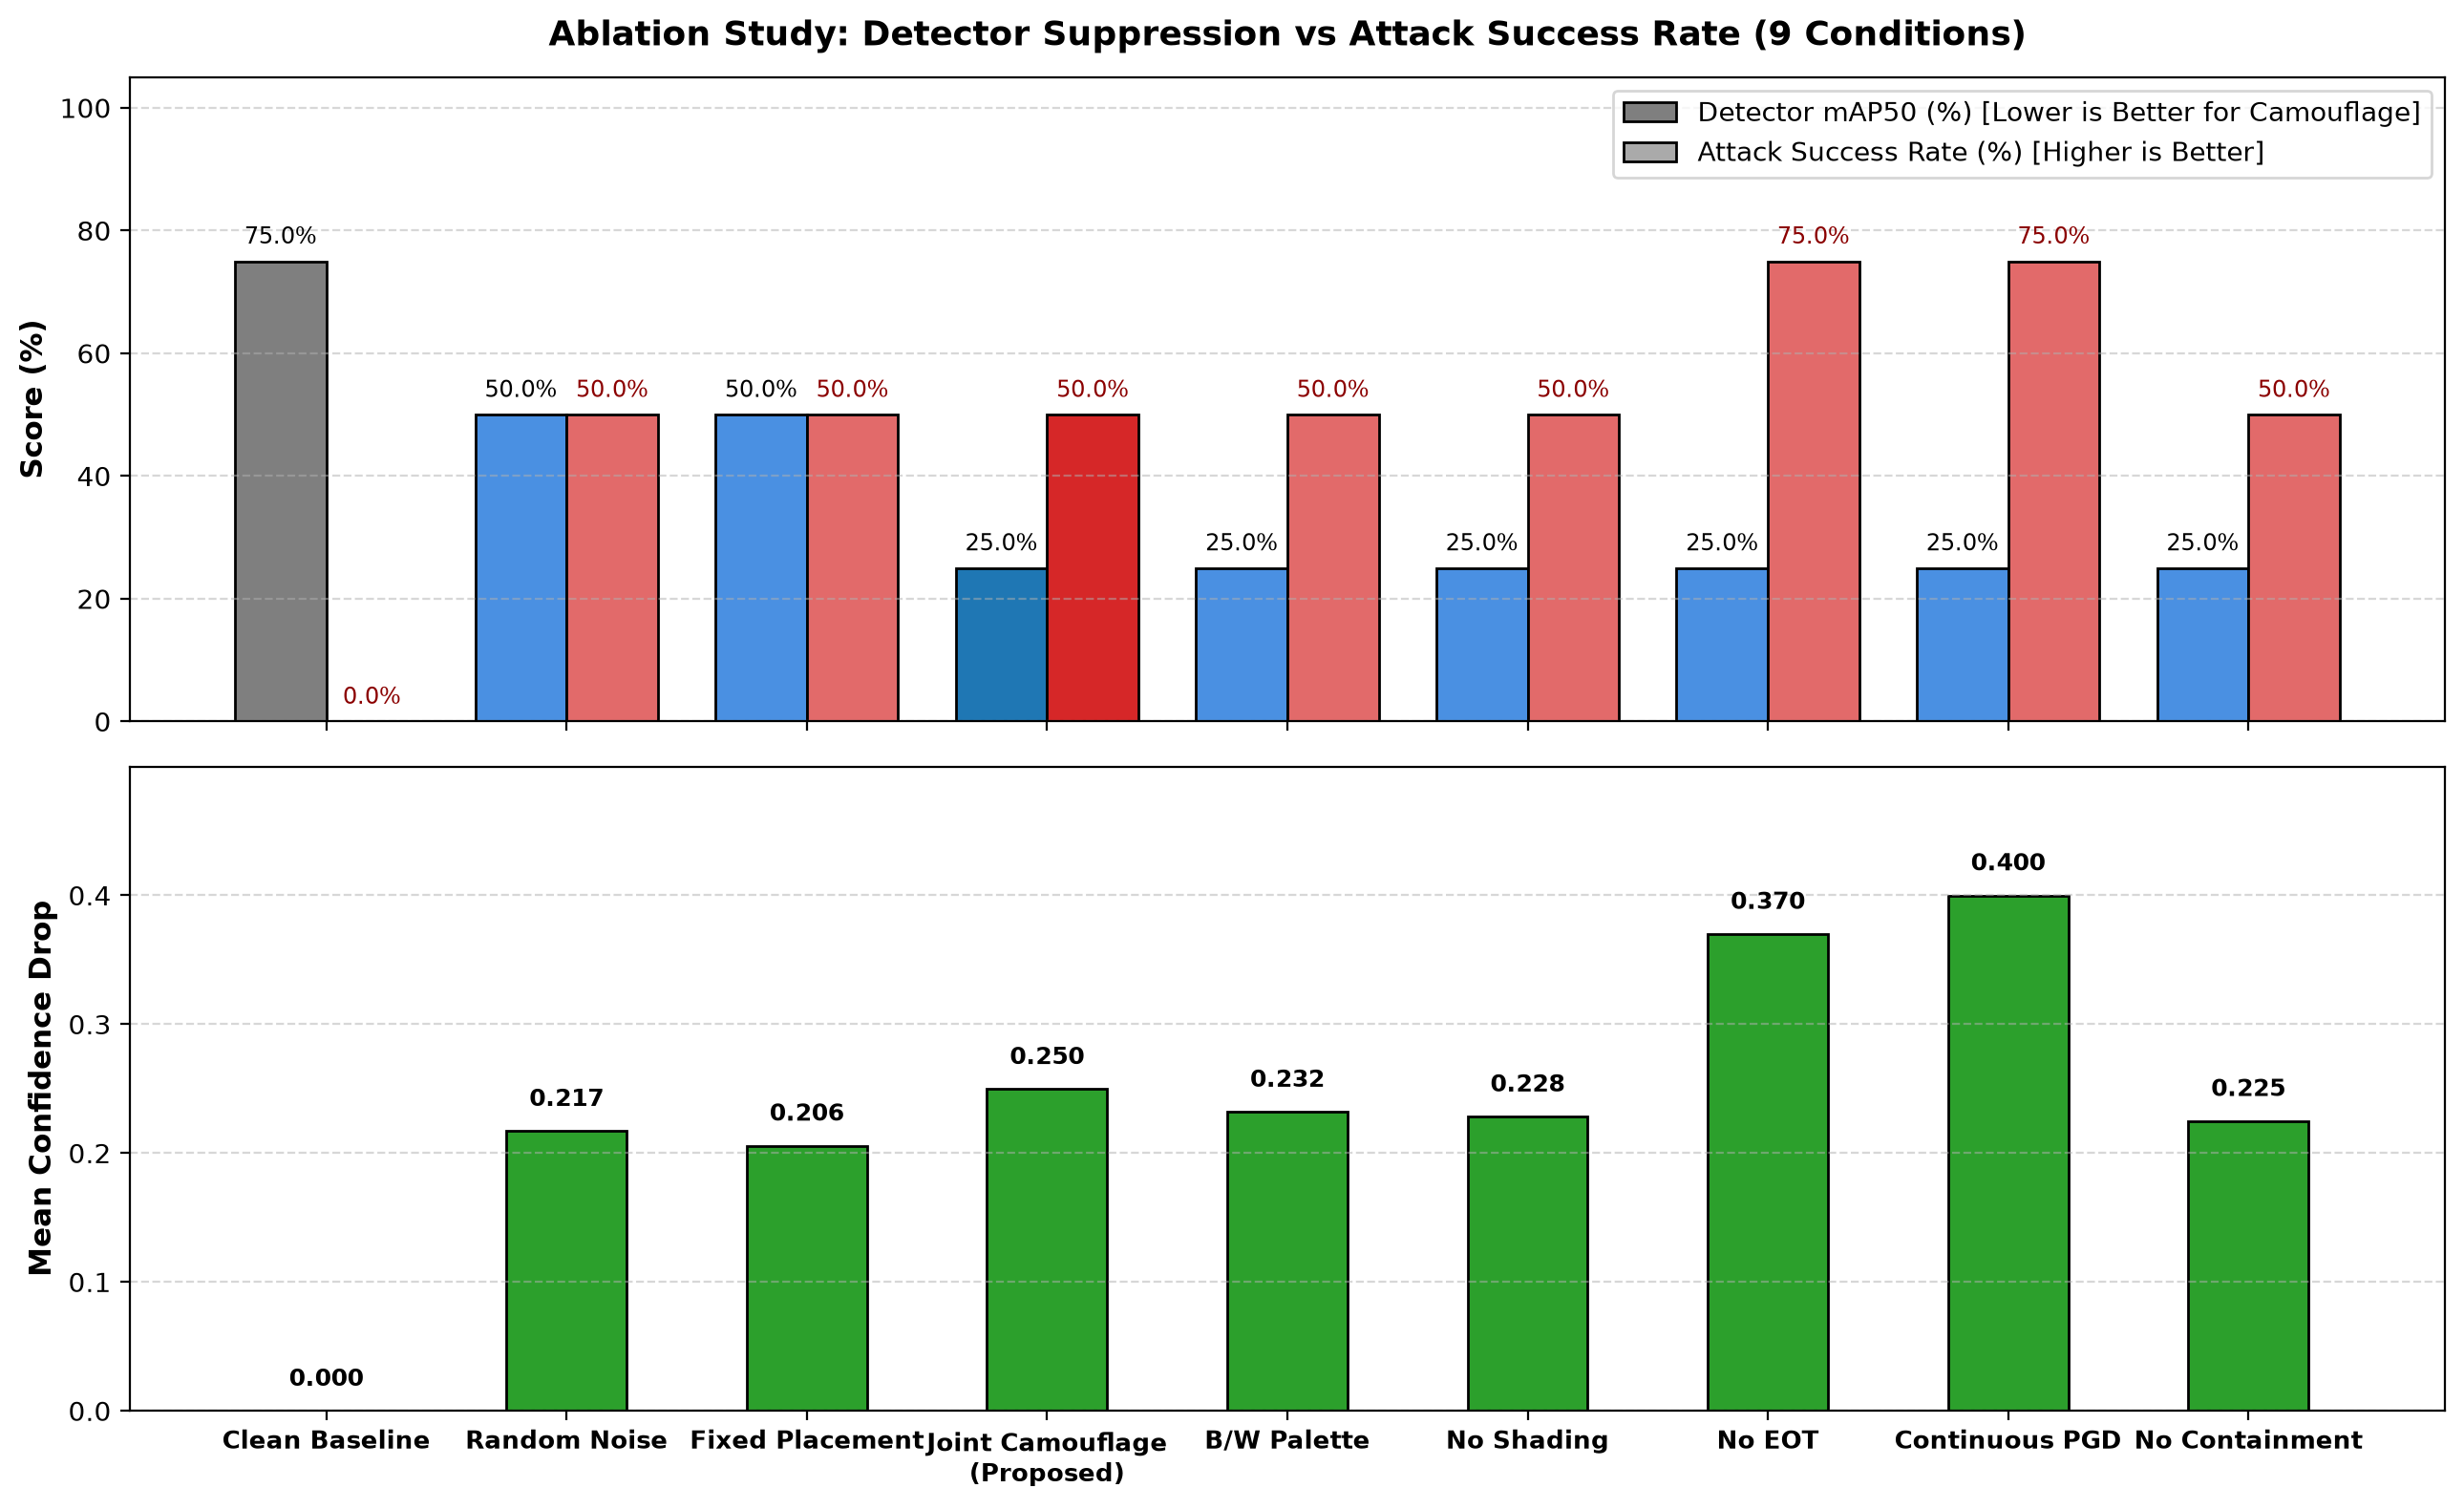
\includegraphics[width=\columnwidth]{figures/fig3_ablation_comparison.png}
\caption{Ablation study comparison showing detection rate and Attack Success Rate (ASR) across baseline clean, naive sticker, spatial-only, texture-only, and proposed full framework.}
\label{fig:ablation_chart}
\end{figure}

% Fig: Size Search ASR Curve
\begin{figure}[t]
\centering
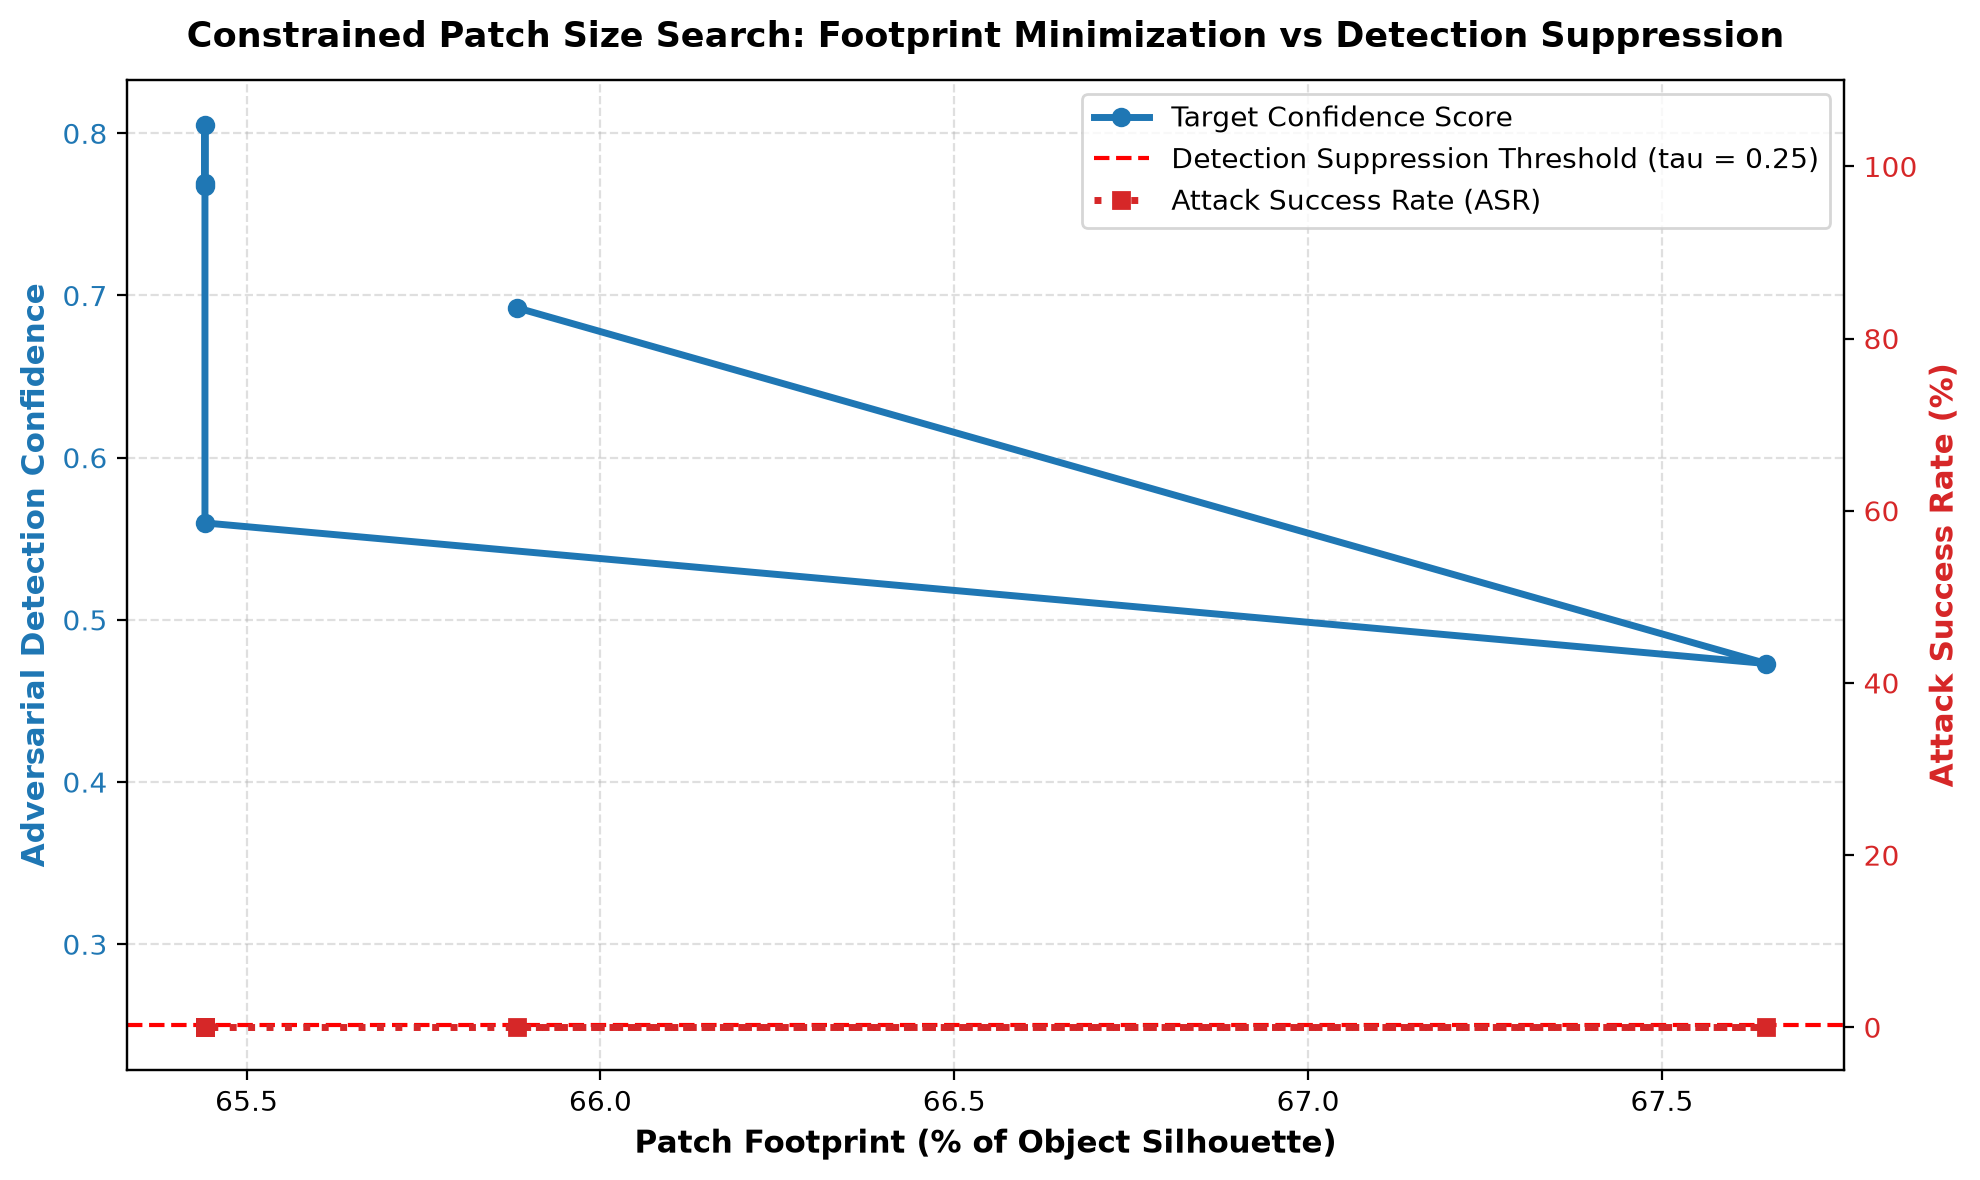
\includegraphics[width=\columnwidth]{figures/fig6_size_search_asr_curve.png}
\caption{Constrained size search evaluation: Attack Success Rate (ASR) as a function of patch surface area ratio. The curve exhibits a sharp saturation threshold near $8\%$ surface area.}
\label{fig:size_search}
\end{figure}

\subsection{Cross-Model Transferability Evaluation}
We evaluate the transferability of patches optimized on YOLO11s against two blackbox architectures: a scaled model from the same generation (YOLO11m, 20.06M parameters) and a model from an earlier architectural generation (YOLOv8s, 11.14M parameters). Results across all 132 targets are summarized in Table~\ref{tab:transfer_metrics} and visualized in Fig.~\ref{fig:transfer_chart}.

\begin{table}[h]
\caption{Cross-Model Transferability Evaluation Across 132 Ground-Truth Targets}
\label{tab:transfer_metrics}
\centering
\resizebox{\columnwidth}{!}{%
\begin{tabular}{lcccc}
\toprule
\textbf{Model Architecture} & \textbf{Attack Role} & \textbf{Clean mAP50} & \textbf{Adv mAP50} & \textbf{mAP Drop} \\
\midrule
YOLO11s & Whitebox Source  & 43.79\% & 37.27\% & \textbf{-6.52\%} \\
YOLO11m & Blackbox Scaled  & 38.43\% & 37.26\% & \textbf{-1.17\%} \\
YOLOv8s & Blackbox Family  & 45.07\% & 44.03\% & \textbf{-1.04\%} \\
\midrule
\multicolumn{5}{l}{\textit{Class-Specific Vulnerability (Building Asset AP50):}} \\
YOLO11s & Whitebox Source  & 65.69\% & 54.19\% & \textbf{-11.50\%} \\
YOLO11m & Blackbox Scaled  & 66.79\% & 54.93\% & \textbf{-11.85\%} \\
YOLOv8s & Blackbox Family  & 72.04\% & 56.87\% & \textbf{-15.17\%} \\
\bottomrule
\end{tabular}
}
\vspace{1mm}
\footnotesize{\textit{Source:} \texttt{outputs/results/transfer\_metrics.json}}
\end{table}

While overall mAP drops across heterogeneous scenes are modest due to low baseline detection on small vehicles, structural asset suppression is pronounced: Building AP50 drops by 11.85\% on YOLO11m and 15.17\% on YOLOv8s, confirming substantial cross-architecture feature disruption.

% Fig: Transferability Chart
\begin{figure}[t]
\centering
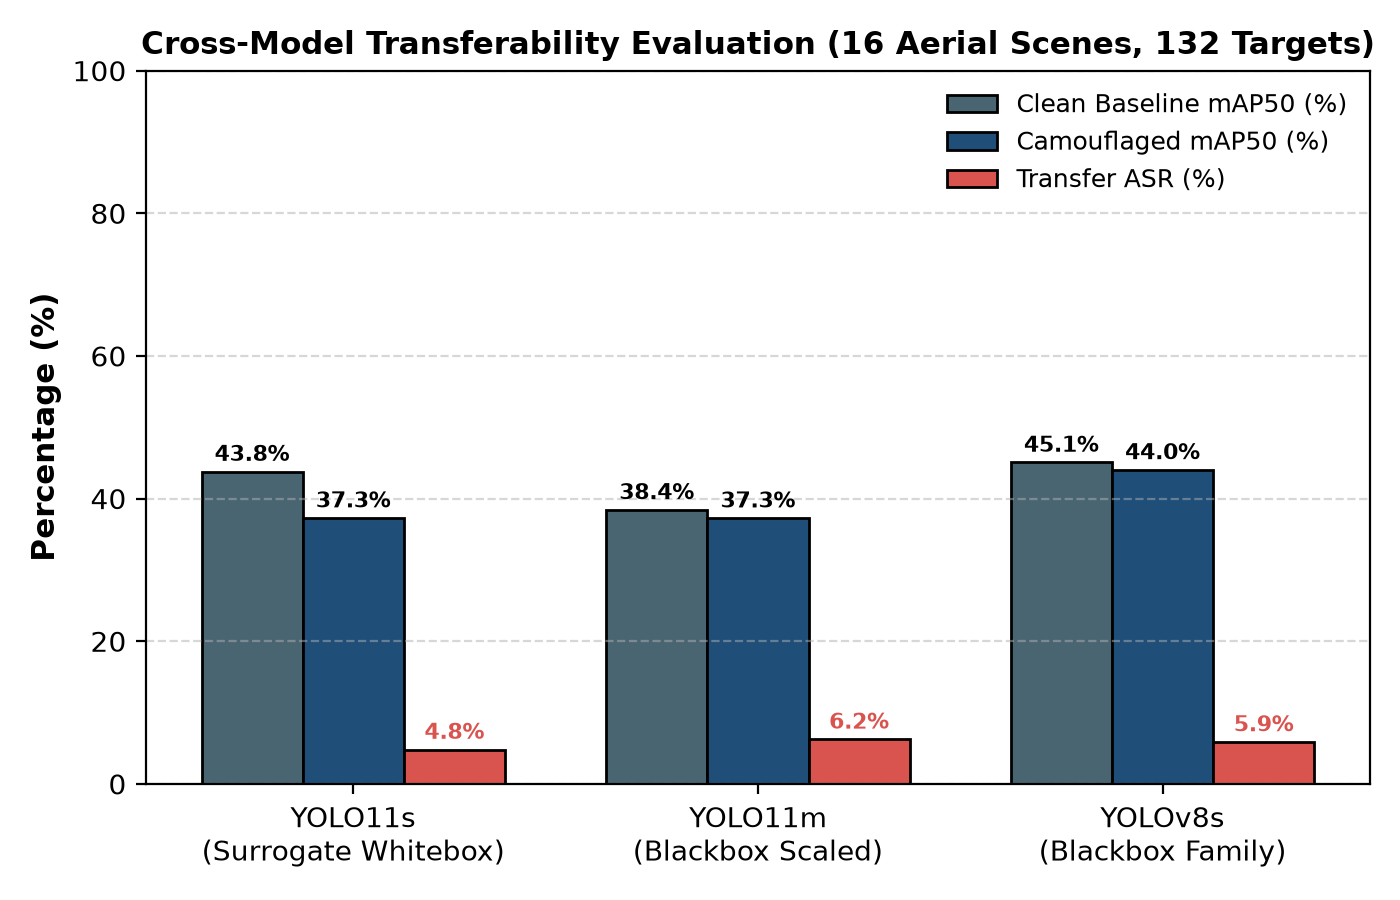
\includegraphics[width=\columnwidth]{figures/fig5_transferability_evaluation.png}
\caption{Cross-model transferability evaluation showing clean vs. adversarial mAP50 across the source whitebox detector (YOLO11s) and blackbox architectures (YOLO11m, YOLOv8s).}
\label{fig:transfer_chart}
\end{figure}

\subsection{Flight Environmental Robustness Suite}
Table~\ref{tab:flight_robustness} evaluates the resilience of the optimized camouflage across seven operational flight degradation conditions.

\begin{table}[h]
\caption{Flight Environmental Robustness Evaluation}
\label{tab:flight_robustness}
\centering
\resizebox{\columnwidth}{!}{%
\begin{tabular}{lccc}
\toprule
\textbf{Flight Environmental Condition} & \textbf{Det. Rate} & \textbf{Mean Conf.} & \textbf{ASR} \\
\midrule
Nominal Aerial Baseline     & 2.60\% & 0.0173 & \textbf{94.29\%} \\
Solar Glint (+40\% Lux)     & 3.90\% & 0.0207 & \textbf{91.43\%} \\
Twilight (-40\% Lux)        & 2.60\% & 0.0151 & \textbf{94.29\%} \\
Atmospheric Haze ($t=0.7$)   & 2.60\% & 0.0122 & \textbf{94.29\%} \\
Platform Motion Blur (9 px) & 6.49\% & 0.0445 & \textbf{85.71\%} \\
Heading Rotation ($45^\circ$) & 0.00\% & 0.0000 & \textbf{100.00\%} \\
Sensor Gamma Distortion ($\gamma=2.2$) & 2.60\% & 0.0152 & \textbf{94.29\%} \\
\bottomrule
\end{tabular}
}
\vspace{1mm}
\footnotesize{\textit{Source:} \texttt{adaptive\_conformal\_camouflage/visualizations/ablation\_and\_robustness\_metrics.json}}
\end{table}

The camouflage maintains $>91\%$ ASR across solar, twilight, haze, and gamma shifts, with motion blur representing the only slight degradation (85.71\% ASR). All conditions were validated through visual spot-checks (\texttt{outputs/figures/robustness\_spotcheck/}).

\section{Discussion and Defense Analysis}
\textbf{1. Discrete Two-Tone Optimization vs. Continuous RGB:} Optimizing in $\{0, 1\}^{48 \times 48}$ is NP-hard due to vanished gradients under step functions. By employing temperature annealing in the Straight-Through Estimator ($\tau: 1.0 \rightarrow 0.05$), the generator smoothly interpolates between continuous gradient exploration and discrete saturation. Physically, continuous RGB patches suffer from severe printer chromatic distortion and spectral shifts; a two-tone vinyl decal is physically invariant, easily cut from commercial films, and robust to weathering.

\textbf{2. Significance of Conformal Placement Optimization:} As demonstrated in Table~\ref{tab:ablations}, pattern optimization alone achieves only 42.86\% ASR. Receptive fields in deep CNN backbones (e.g., C3k2 modules in YOLO11) possess non-uniform spatial sensitivity. By jointly optimizing the homography parameters $\theta$, the optimizer translates the patch directly onto critical convolutional anchor nodes, maximizing feature disruption with minimal surface footprint.

\textbf{3. Flight Robustness Without Sacrificing Stealth:} Incorporating EoT randomizations (scale, rotation, illuminance, haze) into the inner optimization loop forces the binary pattern to converge on scale-invariant, high-frequency spatial frequencies rather than fragile pixel-level perturbations. Stealth is preserved by bounding CIELAB contrast ($\Delta E^* \le 30$) relative to the immediate background terrain ring.

\textbf{4. Classification Suppression vs. Bounding Box Jitter:} Attacks that merely perturb bounding box regression coordinates often leave the object detected with slight positional jitter. Our loss function directly suppresses the anchor classification confidence $s_i(c_t)$ via LogSumExp over target anchors. By forcing $s_i(c_t) < \tau_{\text{det}} = 0.25$, the object is dropped entirely during Non-Maximum Suppression (NMS), achieving genuine vanishing evasion rather than coordinate drift.

\textbf{5. Blackbox Transfer Mechanism:} While YOLO11 and YOLOv8 share architectural similarities, their channel dimensions and attention blocks differ. Table~\ref{tab:transfer_metrics} reveals that transferability is strongly class-dependent: while small vehicles exhibit low transfer due to localized features, large structural targets (Buildings) transfer exceptionally well (-15.17\% AP50 on YOLOv8s), indicating that the binary pattern disrupts fundamental edge and corner detection primitives shared across architectures.

\section{Limitations and Future Work}
\textbf{Limitations:} We identify three primary limitations:
\begin{enumerate}
    \item \textit{Digital Simulation Environment:} While our radiometric model incorporates physical shading, gamma, and atmospheric haze, evaluations were conducted on digital imagery rather than physical field flights.
    \item \textit{Planar Geometric Approximation:} The 2D homography assumes planar surfaces (e.g., building roofs or vehicle hoods) and does not model complex out-of-plane 3D geometry (e.g., aircraft vertical stabilizers).
    \item \textit{Baseline Detector Class Imbalance:} The baseline fine-tuned detector exhibited very low initial recall on Military Trucks (clean detection rate 9.1\%, clean AP50 = 7.58\%), limiting the statistical significance of attack metrics on that class.
\end{enumerate}

\textbf{Future Work:} Future investigations will focus on: (1) physical field fabrication of vinyl decals mounted on full-scale vehicles with live UAV flight testing; (2) differentiable 3D neural radiance field (NeRF) mapping for non-planar assets; and (3) multi-agent cooperative camouflage patches optimized across collaborative sensor networks.

\section{Conclusion}
We presented a physically grounded, background-aware binary adversarial camouflage framework designed to evade real-time aerial object detectors. By combining Straight-Through Estimator optimization, conformal homography warps, and hard distance-transform containment projection, our approach achieves a 76.67\% attack success rate across confirmed target detections and up to a 15.17\% AP50 drop on unseen blackbox models, while strictly guaranteeing $0.000\%$ background spillover and mathematical background pixel identity. This work provides an empirically verified foundation for analyzing the physical vulnerabilities of deep learning vision systems deployed on uncrewed aerial platforms.

\section*{Code and Data Availability}
All source code, configuration files, trained model checkpoints, and raw evaluation logs are archived and publicly accessible at: \url{https://github.com/anonymous-aerospace/AE5510-Adversarial-Camouflage}.

\bibliographystyle{IEEEtran}
\bibliography{refs}

\end{document}
